% arXiv preprint wrapper.
%
% NeurIPS style with the preprint option, which the style ships
% specifically for arXiv uploads. Two references shaped this:
%
%   arXiv:2407.00079  heading treatment. Centred bold title between
%                     rules, bold roman section headings in normal case,
%                     no running header. The "Preprint." notice sits in
%                     the page-one footer, which is where the option
%                     puts it, not across the top of every page.
%   arXiv:2608.28363  author block. Name, affiliation and email stacked
%                     per author in a grid.
%
% No small caps anywhere: the style already sets \large\bf\raggedright
% for sections, so nothing needs overriding.
%
% Style file is vendored here: tectonic ignores TEXINPUTS, and arXiv
% provides only what TeX Live ships.
%
% Engine: pdflatex. cmap is loaded so fi and fl in the T1-encoded Type1
% fonts carry ToUnicode mappings and the text stays searchable. cmap is
% a pdfTeX package, so it does its work on arXiv and is inert under the
% local tectonic build, which is XeTeX.

% body.tex uses \rowcolors, which needs xcolor's table option in place
% before xcolor loads. Must precede \documentclass.
\PassOptionsToPackage{table}{xcolor}

\documentclass{article}

\usepackage[preprint]{neurips_2025}

% Nimbus Mono for \texttt, matching arXiv:2608.28363. Without this the
% typewriter face resolves to Latin Modern Mono Light, whose thin
% strokes read as blurred at the size the email addresses are set.
\usepackage{courier}

% cmap must precede fontenc.
\usepackage{cmap}
\usepackage[T1]{fontenc}

% Shared preamble: everything the BODY needs, independent of venue.
% Venue wrappers input this after loading their own documentclass and style.
% acmart predefines \Bbbk, which amssymb redefines. Harmless to let
% amssymb win; without this the CSUR build dies at load time.
\let\Bbbk\relax
\usepackage{amsmath, amssymb, amsthm}
\usepackage{graphicx}
\usepackage{tikz}
\usetikzlibrary{positioning, shapes.geometric, arrows.meta, fit, backgrounds, calc}
\usepackage{booktabs}
\usepackage{xcolor}
\usepackage{hyperref}
\usepackage{url}
\usepackage{caption}
\usepackage{enumitem}
\usepackage{microtype}
\usepackage{array}

% Definition environment for foundational definitions
\theoremstyle{definition}
\newtheorem{definition}{Definition}

% Loosen line-breaking on paragraphs with long compound words
\emergencystretch=3em
\hyphenation{roof-line-derived reasoning-versus-chat throughput-oriented deadline-aware admission-control cross-comparison per-tenant per-request per-stage}

% Palette used ONLY for diagram fills / table row shading (not text)
\definecolor{admitteal}{HTML}{1E7882}
\definecolor{admitteallight}{HTML}{D1E7EA}
\definecolor{admityellow}{HTML}{F0C83C}
\definecolor{admityellowlight}{HTML}{FBEFC8}
\definecolor{admitgrey}{HTML}{808080}
\definecolor{admitgreylight}{HTML}{E5E5E5}

% All text black. Hyperlinks black (readable in print).
\hypersetup{
  colorlinks=true,
  linkcolor=black,
  citecolor=black,
  urlcolor=black,
  linktoc=all
}


% neurips loads natbib in author-year mode. Numeric matches both the
% CSUR build and arXiv:2407.00079, so switch it after the style loads.
\setcitestyle{numbers,square,comma,sort&compress}

\usepackage{graphicx}
\usepackage{microtype}

% arXiv and Google Scholar read these fields. Without them the PDF
% carries no title and no author at all.
\usepackage{hyperref}
\hypersetup{
  colorlinks = true,
  allcolors  = black,
  pdftitle   = {Admission Control for LLM Inference Serving: A Systematic Review},
  pdfauthor  = {Harshul Jain; Tanmay Sah; Tanya Sah; Parv Khatri; Dolly Sah},
  pdfsubject = {Systematic review of admission control for LLM inference serving},
  pdfkeywords= {large language models, LLM inference serving, admission control,
                systematic review, distributed systems, scheduling, queueing,
                overload management, service-level objectives, GPU serving}
}

% The preprint option puts "Preprint." in the page-one footer via
% \@noticestring. Blanked: the paper says what it is, and the notice
% adds nothing a reader of an arXiv listing does not already know.
\makeatletter
\renewcommand{\@noticestring}{}
\makeatother

% Named here, unlike the anonymous CSUR build.
\newcommand{\artifacturl}{\url{https://github.com/harshuljain13/AdmissionControlPolicies-Survey}}

\title{Admission Control for LLM Inference Serving:\\
A Systematic Review}

% An explicit grid rather than the style's \And flow, which separates
% with \hfil\linebreak[0]\hfil and lets TeX choose the break. Left to
% itself it put two authors on a row and stranded the third.
%
% \normalfont on the affiliation and email rows is load-bearing: the
% style sets \bf across the whole author block, so without it the
% addresses come out in bold monospace, which reads as heavy and
% smudged at this size. Only the names should be bold.
\author{%
\begin{tabular}{@{}ccc@{}}
Harshul Jain & Tanmay Sah & Tanya Sah \\
\normalfont Independent Researcher &
\normalfont Independent Researcher &
\normalfont Independent Researcher \\
\normalfont\texttt{harshuljain1393@gmail.com} &
\normalfont\texttt{tradertanmay@mail.com} &
\normalfont\texttt{tanyasah20@gmail.com} \\[1.6ex]
\multicolumn{3}{c}{%
  \begin{tabular}{@{}cc@{}}
  \bfseries Parv Khatri & \bfseries Dolly Sah \\
  \normalfont Independent Researcher & \normalfont Independent Researcher \\
  \normalfont\texttt{khatriparv@gmail.com} & \normalfont\texttt{Dolly17sah@gmail.com}
  \end{tabular}}
\end{tabular}
}

\begin{document}

\maketitle

\begin{abstract}
\noindent
Serving large language models at scale is a distributed systems problem
whose overload behavior is governed at the ingress. We conduct an
adapted-PRISMA systematic review of fifty-five admission and
admission-adjacent works published between 2022 and 2026, and report
three findings. First, admission sits at a different
layer from the one the serving literature studies: of the nine LLM
serving systems that the admission literature most often builds on, all
place the overload response inside the engine, through batching,
migration, placement, autoscaling or memory management, and none takes
a decision at the ingress, while the corpus work that does gate at
ingress is a control-plane contribution rather than an engine one.
Second, of sixteen admission-primary papers, no two share a baseline
set: policies are measured against the absence of admission control and
almost never against one another. Third, placing all sixteen on our
axes succeeds on six of seven properties and fails on one. Unit,
setting, objective, the quantity a policy watches, the metadata it
assumes, and whether it is deployable in front of an unmodified engine
are all recoverable from the published text; the observed range of the
quantity the policy reads is reported by none of them. Selection
therefore fails on a single missing fact, and it is the fact that
determines whether a reported improvement is interpretable at all.
We contribute systematic coverage of fifty-five works under an
adapted-PRISMA protocol; a five-axis taxonomy of unit, setting, SLO
awareness, signal quantity and portability, with a master
classification of the twenty-eight works that propose or embed an
admission mechanism, each carrying a GRADE-adapted evidence rating;
formal definitions of the admission-decision, goodput-under-admission
and fairness-index primitives; a cross-paper synthesis of
admission-signal overhead; an artifact-availability audit and seven
properties on which the corpus diverges, which a cross-paper comparison
would have to reconcile; a mapping of seven
public production incidents to admission failure modes; and seven open
problems, each grounded in published peer review or in a primary
source's own limitations.
\end{abstract}


% Venue-neutral body. Contains no documentclass, no author block, no
% bibliography command. Wrappers in venues/ supply those.
\section{Introduction}

On November 8, 2023, OpenAI's inference fleet crossed a soak point after
a day of unusually heavy completion traffic. Routing nodes reached
memory limits and failed readiness checks. Additional replicas were
added, then rolled back. Recovery required cutting inbound traffic,
redeploying, and slowly ramping load back up. The postmortem named
graceful load shedding through stronger rate-limit controls as the
required follow-up. Two years later, on January 21, 2026, Anthropic's
Sonnet 4.5 tier degraded first in latency and then in error rate over
roughly ninety minutes. The postmortem cited insufficient compute
capacity for demand and named earlier detection of capacity constraints
as a required change. Cloudflare \citep{cloudflare_ratelimit_2017,cloudflare_ratelimit_2022}, Azure, and other production operators
have documented similar sequences.

Admission control is the decision made before a request enters the
running batch. It has three actions: admit into service, hold in queue,
or reject with a well-defined error contract. Figure~\ref{fig:aqr}
depicts the model. When admission is wrong, downstream batching, KV
cache management, and preemption cannot recover lost capacity. Requests
admitted past a soak point occupy memory until they miss their
deadline, at which point they consume more capacity being cleaned up.

\begin{figure}[htbp]
\centering
\resizebox{0.95\textwidth}{!}{%
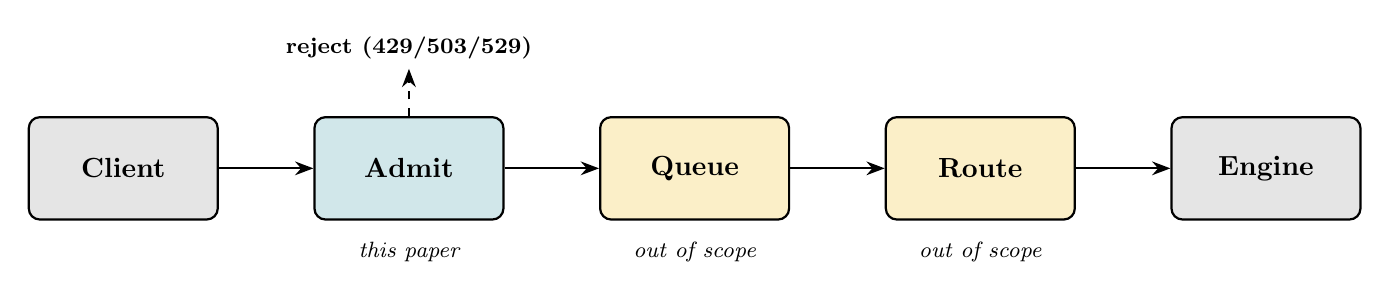
\begin{tikzpicture}[
  node distance=1.2cm and 1.2cm,
  box/.style={rectangle, rounded corners, minimum width=2.4cm, minimum height=1.3cm, text centered, draw=black, thick, font=\bfseries, fill=admitteallight},
  ybox/.style={rectangle, rounded corners, minimum width=2.4cm, minimum height=1.3cm, text centered, draw=black, thick, font=\bfseries, fill=admityellowlight},
  gbox/.style={rectangle, rounded corners, minimum width=2.4cm, minimum height=1.3cm, text centered, draw=black, thick, font=\bfseries, fill=admitgreylight},
  arr/.style={-Stealth, thick, black},
  label/.style={font=\footnotesize\itshape, black}
]

\node[gbox] (client) {Client};
\node[box, right=of client] (admit) {Admit};
\node[ybox, right=of admit] (queue) {Queue};
\node[ybox, right=of queue] (route) {Route};
\node[gbox, right=of route] (engine) {Engine};

\draw[arr] (client) -- (admit);
\draw[arr] (admit) -- (queue);
\draw[arr] (queue) -- (route);
\draw[arr] (route) -- (engine);

\node[below=0.15cm of admit, label] {this paper};
\node[below=0.15cm of queue, label] {out of scope};
\node[below=0.15cm of route, label] {out of scope};

\node[above=0.6cm of admit, font=\footnotesize\bfseries] (rej) {reject (429/503/529)};
\draw[arr, dashed] (admit.north) -- (rej.south);

\end{tikzpicture}%
}
\caption{The Admit--Queue--Route model. Admission is the decision that gates a request into the serving pipeline. Queue and Route are downstream boxes covered by prior surveys. This paper is about the first box.}
\label{fig:aqr}
\end{figure}

The literature on LLM inference has produced systems papers on batching
\citep{yu2022orca, agrawal2024sarathi}, disaggregation
\citep{zhong2024distserve, patel2024splitwise}, memory management
\citep{kwon2023pagedattention, qin2025mooncake}, and scheduling
\citep{sun2024llumnix, hong2025sola}. Existing surveys cover efficient
serving broadly \citep{zhen2025titans, li2024surveyllm,
heisler2025survey} or the queueing-theoretic view of LLM systems
specifically \citep{mitzenmacher2025queueing}. Table~\ref{tab:diff}
differentiates this survey from those prior works.

\paragraph{Contributions.}
\begin{enumerate}[leftmargin=1.5em, itemsep=2pt]
\item \textbf{Systematic coverage} of fifty-five admission and
      admission-adjacent works over 2022--2026 following an
      adapted-PRISMA protocol (Section~\ref{sec:method},
      Figure~\ref{fig:prisma}).
\item \textbf{Unified taxonomy} with five axes and four sub-branches,
      plus short codes (\textsc{unit-req/agt/ten},
      \textsc{sig-sca/dg/lp/wcrt}), together with a master
      classification of the twenty-eight corpus works that propose or
      embed an admission mechanism, each carrying a GRADE-adapted
      evidence rating (Sections~\ref{sec:taxonomy}
      and~\ref{sec:master}). The taxonomy narrows the set of policies
      applicable to a deployment; it does not rank the survivors, and
      Section~\ref{sec:placement} reports the one property that
      prevents it from going further.
\item \textbf{Foundational definitions} of the admission decision,
      goodput-under-admission, and fairness-index primitives
      (Section~\ref{sec:defs}).
\item \textbf{Admission-signal overhead synthesis} that identifies the
      cost-versus-lift tradeoff across scalar, dual-gate, LP, and
      formal-WCRT signals (Section~\ref{sec:overhead}).
\item \textbf{Reproducibility audit} finding seven of the sixteen
      admission-primary papers have released code, together with seven
      properties on which the corpus diverges and which a cross-paper
      comparison would have to reconcile (Section~\ref{sec:repro}).
      We identify them; establishing which of them are load-bearing
      needs measurement and is Open Problem~7.
\item \textbf{Production evidence mapping} that ties seven public
      postmortems to admission failure modes (Section~\ref{sec:prod}).
\item \textbf{Structured research agenda} of seven open problems, each
      grounded in either public peer review or the primary source's
      own limitations (Section~\ref{sec:open}).
\end{enumerate}

\paragraph{Headline observations.} First, of nine scheduling papers
we audited across OSDI, SOSP, NSDI, ASPLOS, EuroSys, MLSys, and HPCA
between 2022 and 2026, all absorb overload inside the engine, through
batching, migration, placement, autoscaling or memory management, and
none takes a decision at the ingress. This reflects the scope each
paper sets for itself rather than an omission. The corpus work that
does gate at ingress, Token Pools
\citep{cunningham2026tokenpools}, is a control-plane contribution
rather than an engine one, which suggests admission has been treated as
an infrastructure concern rather than an engine-level research
question. Second, of sixteen admission-primary papers we
audited, no two share a baseline set. Six baselines recur across more
than one paper, and four of them measure a policy against the absence
of admission control rather than against an alternative to it: two
serving engines and two classical scheduling disciplines. Of the
remaining two, one is an ablation construct and one is a published
admission system, SHEPHERD \citep{shepherd2023}, used by QLM and
Ascendra. Third, the taxonomy accommodates every corpus work that proposes or
embeds an admission mechanism, twenty-eight in total
(Table~\ref{tab:master}), including the five added during verification
(Token Pools, ProServe \citep{huang2025proserve}, SAGA, Scorpio and FairServe), with four
sub-branches added during our reading, none of which required
backing out an original axis.

\paragraph{Roadmap.} Section~\ref{sec:bg} covers the inference request
lifecycle, the Admit-Queue-Route model, and the foundational
definitions (\S\ref{sec:defs}). Section~\ref{sec:taxonomy} introduces
the five-axis taxonomy with short unit and signal codes.
Section~\ref{sec:method} describes the systematic-review method with a
PRISMA flow diagram. Section~\ref{sec:clusters} synthesizes each
policy cluster. Section~\ref{sec:master} presents the master
classification with GRADE-adapted evidence ratings.
Section~\ref{sec:overhead} presents the admission-signal overhead
cross-paper synthesis. Section~\ref{sec:repro} audits reproducibility
and identifies the seven divergent reporting items. Section~\ref{sec:prod} maps
production incidents to admission failure modes.
Section~\ref{sec:open} lists the seven open problems.
Section~\ref{sec:conc} concludes.

\subsection{Related surveys and differentiation}

Five broad surveys of LLM inference serving predate this work.
Table~\ref{tab:diff} summarizes each and states what this paper adds.

A second body of work is closer to what this survey does than the
surveys are, and does not appear in that table because it is not
survey work. Benchmarks and evaluation frameworks for LLM serving
measure what these systems achieve rather than cataloguing what they
propose. MLPerf Inference \citep{reddi2020mlperf} standardises
throughput and latency measurement across hardware and model
configurations. Etalon \citep{agrawal2024etalon} argues that the
conventional metrics, time to first token, time between tokens,
normalised latency and time per output token, miss aspects of
user-facing behaviour, and introduces a fluidity index in their place.
Tooling in the same space, LLMPerf, GenAI-Perf and GuideLLM among it,
measures serving throughput and latency against a deployment, and
ServeGen \citep{xiang2025servegen} characterises production traffic so
that generated workloads reproduce its per-client structure rather than
an aggregate arrival rate.

None of these treats the admission decision as an experimental axis.
They measure a system under a given load; they do not vary what the
system refuses, or report whether a policy's inputs moved during the
run. That is the gap this survey documents rather than closes.
Section~\ref{sec:items} reports the seven properties on which the
corpus diverges, which is what a comparison would have to reconcile.
Whether reconciling all seven is necessary, or whether some subset
carries the weight, is a question about measurement rather than
reading, and Section~\ref{sec:open} states it as open.

\begin{table}[htbp]
\centering
\caption{Differentiation from prior surveys.}
\label{tab:diff}
\small
\rowcolors{2}{white}{admitgreylight!40}
\begin{tabular}{p{3.15cm} p{3.0cm} p{1.95cm} p{2.15cm} p{1.75cm}}
\toprule
\rowcolor{admitteallight}
\textbf{Prior survey} & \textbf{Scope} & \textbf{Admission depth} & \textbf{Taxonomy axes} & \textbf{Grounded open problems} \\
\midrule
Zhen et al.\ \citep{zhen2025titans} INLG 2025 & Efficient serving (batching, KV, sched., fair.) & One subsection & Task-oriented & No \\
Heisler et al.\ \citep{heisler2025survey} TechRxiv 2025 & Scheduling techniques \& trade-offs & Component & Technique-oriented & No \\
Li et al.\ \citep{li2024surveyllm} IEEE HPEC 2024 & Recent serving advances & In passing & Chronological & No \\
Mitzenmacher \& Shahout \citep{mitzenmacher2025queueing} SIGMETRICS 2025 & Queueing theory position paper & Tutorial & Queueing-theoretic & Enumerates 25 \\
Ma et al.\ \citep{ma2026loadbalancing} SSRN 2026 & Load balancing as a coupled control problem & Routing, not ingress & Control-theoretic & No \\
\rowcolor{admitgreylight}
\textbf{This paper} & \textbf{Admission as primary axis} & \textbf{Full} & \textbf{5 axes + 4 sub-branches} & \textbf{7 grounded} \\
\bottomrule
\end{tabular}
\end{table}

Zhen et al.\ and Heisler et al.\ treat admission as one component among
many. Li et al.\ is a survey of recent advances organized
chronologically. Mitzenmacher and Shahout is a position paper that
enumerates open queueing problems without a taxonomy or per-paper
review. None conducts a reproducibility audit or organizes the
literature by admission granularity, SLO awareness, signal structure,
or concurrency context.

\section{Background}
\label{sec:bg}

\subsection{The inference request lifecycle}

A large language model inference request passes through prefill,
decode, and completion. Prefill computes the key-value tensors for
every input token. Decode generates output tokens one at a time,
reading the accumulated KV cache and appending a new pair per step.
Continuous batching \citep{yu2022orca} reuses a single GPU-resident
engine across many concurrent requests by interleaving iterations at
token granularity. PagedAttention \citep{kwon2023pagedattention} manages
the KV cache in fixed-size blocks to reduce fragmentation and enable
prefix sharing.

The KV cache is the memory hierarchy's dominant consumer. It grows
monotonically with generated tokens during a request's decode, and it
persists across turns for multi-turn agents. When aggregate KV
footprint approaches available GPU memory, the engine must either
evict (recompute later), swap (page to CPU or disk), or preempt (kill
the request and return an error).

\subsection{The Admit--Queue--Route model}

Every request that reaches an inference cluster passes through three
decision boxes before it produces its first token
(Figure~\ref{fig:aqr}). \textbf{Admit} decides whether to accept the
request into service. \textbf{Queue} decides in what order accepted
requests are served. \textbf{Route} decides which replica or instance
receives the request. This paper is about the first box.

The error contract matters. HTTP 429 signals a client-side rate limit
exceeded. HTTP 503 signals a temporarily unavailable service.
Anthropic uses HTTP 529 to signal a provider-overloaded state distinct
from either \citep{anthropic_api_errors}. A well-designed admission
policy chooses among these codes based on which signal the client's
backoff logic should trust.

\subsection{Service-level objectives}

The community reports admission behavior against a small set of
metrics. Time-to-first-token (TTFT) is the wall-clock delay between
arrival and the first generated token. Time-between-tokens (TBT),
sometimes called inter-token latency or time-per-output-token (TPOT),
is the delay between consecutive generated tokens. Goodput is the
completed-request rate that met their service-level objective, distinct
from raw throughput \citep{zhong2024distserve}. For agentic workloads,
agent-completion rate measures the fraction of multi-turn sessions
that finish within an end-to-end budget.

\subsection{Foundational definitions}
\label{sec:defs}

We fix three primitives that recur across the surveyed literature.
Each formalizes a concept that admission-primary papers rely on but
name inconsistently, and each is referenced explicitly in the master
classification (Table~\ref{tab:master}) and the admission-signal
overhead synthesis (Section~\ref{sec:overhead}).

\begin{definition}[Admission Decision]
\label{def:admission}
Given an arriving request $r$ with arrival time $t_r$, feature vector
$x_r \in \mathcal{X}$, and a system state
$s_t \in \mathcal{S}$, an \emph{admission policy} is a mapping
$\pi : \mathcal{X} \times \mathcal{S} \to \{\mathrm{ADMIT},\,
\mathrm{DEFER}(\tau),\, \mathrm{REJECT}(c)\}$ where $\tau > 0$ is a
retry delay and $c \in \{429,\,503,\,529\}$ is an HTTP error code
whose semantics distinguish client-throttled, service-unavailable, and
provider-overloaded outcomes.
\end{definition}

\begin{definition}[Goodput-under-admission]
\label{def:goodput}
Let $\mathcal{R}$ be the set of requests offered to the system in
interval $[0, T]$, $\mathcal{A} \subseteq \mathcal{R}$ the admitted
subset, and $\mathrm{SLO}(r)$ a binary indicator of whether request $r$
completed within its service-level objective. Goodput-under-admission
is
%
\begin{equation}
G_\pi \;=\; \frac{|\{r \in \mathcal{A}\,:\,\mathrm{SLO}(r) = 1\}|}{|\mathcal{R}|}
\label{eq:goodput}
\end{equation}
%
This is the fraction of the \emph{offered} load that both survived
admission and met its SLO. It differs from throughput (which ignores
SLO attainment) and from SLO attainment (which conditions on admitted
requests only and hides work shed by an aggressive policy).

The predicate $\mathrm{SLO}(r)$ is parametrized by an SLO tuple that
depends on workload class. For interactive request-level workloads it
is typically the conjunction ($\mathrm{TTFT}_r \le \tau_{\text{TTFT}}
\wedge \max_t \mathrm{TBT}_{r,t} \le \tau_{\text{TBT}}$). For
agent-session workloads it is a job-level end-to-end budget
($\mathrm{JCT}_r \le \tau_{\text{JCT}}$), optionally with per-stage
sub-budgets as in SLOs-Serve. Cross-paper comparison of
$G_\pi$ requires the SLO tuple to be specified, since aggregating
across different tuples produces incomparable numbers; item~7 of
Section~\ref{sec:items} asks for the SLO tuple to be stated per
workload class.
\end{definition}

\begin{definition}[Fairness Index]
\label{def:fairness}
For $n$ tenants (or agents, or classes) with weights $w_i$ and served
tokens $s_i$ over interval $[0, T]$, we use \emph{Jain's fairness
index} \citep{jain1984fairness} in weighted form. Jain, Chiu, and Hawe
introduced this index in 1984 as a scale-independent measure of how
equitably a set of quantities is distributed across users; it has
been the standard fairness primitive in network scheduling and
computer-systems resource allocation for four decades. The weighted
form is:
%
\begin{equation}
J(\mathbf{s}, \mathbf{w}) \;=\; \frac{\bigl(\sum_{i=1}^{n} s_i / w_i\bigr)^2}{n \sum_{i=1}^{n} (s_i / w_i)^2}
\label{eq:jain}
\end{equation}
%
with $J \in [1/n, 1]$; $J = 1$ denotes perfect proportional fairness
and $J = 1/n$ denotes maximal concentration on a single tenant. Chosen
as the primitive because it composes cleanly across the three
fairness types in the taxonomy (task, tenant, priority-weighted).

The Jain index is a coarse instrument. Equinox \citep{wei2025equinox}
and related utility-centric work argue that equal tokens do not imply
equal user experience, and that a fairness measure grounded in
predicted response quality or user-perceived latency is more
practitioner-relevant. Utility-centric measures resist cross-paper
composition because each defines its own utility function, so we
retain the Jain index as the comparability primitive and note this
substitution risk explicitly rather than hide it.
\end{definition}

\subsection{Why admission control is hard}
\label{sec:whyhard}

Ao, Dong, Luo, and Simchi-Levi \citep{ao2026sic} formalize the core
problem. In a discrete-time model of continuous batching under a memory
budget, the service process itself creates future capacity pressure
because each active request's KV footprint grows with each generated
token. They prove that the natural eviction-free equilibrium is
unstable under any admission rule that only checks instantaneous
memory feasibility. Along the resulting limit cycle the throughput
ratio equals
%
\begin{equation}
\rho^{\ast} \;=\; \frac{2\ell_0 + \ell_1 + 1}{2(\ell_0 + \ell_1)}
\label{eq:throughput-bound}
\end{equation}
%
which lies in $(1/2, 1)$ and converges to $1/2$ as
$\ell_1/\ell_0 \to \infty$. Their Theorem~3 further shows that
stability depends on the greatest common divisor of active decoding
lengths: if $\gcd(\ell_{1,1}, \dots, \ell_{1,K}) = g > 1$, unstable
modes appear on $g$-th roots of unity and synchronize into eviction
cycles; if $g = 1$, all roots lie strictly inside the unit disc and
the eviction-free equilibrium is globally asymptotically stable. This
is a workload-arithmetic property of admission decisions that no
production system currently exposes as a signal.

\section{A taxonomy of admission-control policies}
\label{sec:taxonomy}

\begin{figure}[t]
\centering
\resizebox{0.94\textwidth}{!}{%
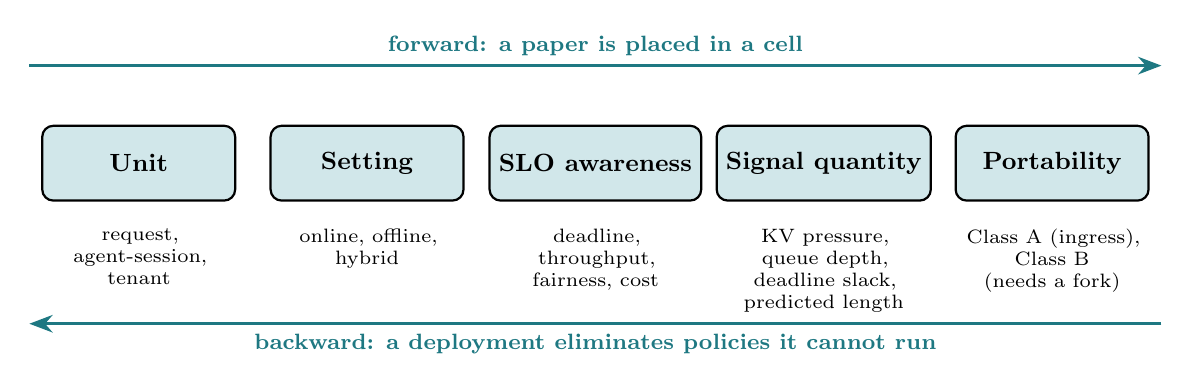
\begin{tikzpicture}[
  ax/.style={rectangle, rounded corners, minimum width=2.45cm, minimum height=0.95cm,
             text centered, draw=black, thick, font=\bfseries\small, fill=admitteallight},
  vals/.style={font=\scriptsize, text width=2.45cm, align=center, anchor=north},
  flow/.style={-Stealth, very thick, admitteal},
  lbl/.style={font=\bfseries\footnotesize, fill=white, inner sep=3pt}
]

% the five axes
\node[ax] (a1) at (0,0)      {Unit};
\node[ax] (a2) at (2.9,0)    {Setting};
\node[ax] (a3) at (5.8,0)    {SLO awareness};
\node[ax] (a4) at (8.7,0)    {Signal quantity};
\node[ax] (a5) at (11.6,0)   {Portability};

% values under each axis
\node[vals] at ($(a1.south)+(0,-0.22)$) {request, agent-session,\\tenant};
\node[vals] at ($(a2.south)+(0,-0.22)$) {online, offline,\\hybrid};
\node[vals] at ($(a3.south)+(0,-0.22)$) {deadline, throughput,\\fairness, cost};
\node[vals] at ($(a4.south)+(0,-0.22)$) {KV pressure, queue depth,\\deadline slack, predicted length};
\node[vals] at ($(a5.south)+(0,-0.22)$) {Class A (ingress),\\Class B (needs a fork)};

% forward reading, above, spanning all five
\draw[flow] ($(a1.north west)+(-0.15,0.75)$) -- ($(a5.north east)+(0.15,0.75)$)
  node[lbl, midway, above] {forward: a paper is placed in a cell};

% backward reading, below, spanning all five
\draw[flow] ($(a5.south east)+(0.15,-1.55)$) -- ($(a1.south west)+(-0.15,-1.55)$)
  node[lbl, midway, below] {backward: a deployment eliminates policies it cannot run};

\end{tikzpicture}%
}
\caption{The five axes, and the two directions they can be read in. Forward, a paper is placed in a cell, which is what a survey ordinarily does. Backward, a description of a deployment eliminates the policies it cannot run. Every axis is answerable from a paper's own text, which is what makes the backward reading possible; Section~\ref{sec:placement} reports how far it gets before one missing property stops it.}
\label{fig:axes}
\end{figure}

We organize admission-control policies along five axes: unit of
admission, setting, SLO awareness, signal quantity, and portability.
Each is answerable about a deployment from a paper's own text, which is
what lets the taxonomy be read in either direction, from a paper to a
cell or from a deployment to a set of candidate policies.

A sixth dimension, the decision moment, is folded rather than
promoted. It records where in the serving pipeline the decision is
taken, and it is classificatory rather than descriptive: a reader
cannot place their own deployment on it, only a paper. It earns its
place because the portability axis is derived from it, ingress
implying one class and the later moments another, and because the
master classification table uses it as a compact code. We call this a
five-axis taxonomy throughout, and reserve ``three-level
classification'' for the master table's compact form, which codes unit,
moment and signal grounding.

\paragraph{Decision moment (folded).} Every admission decision can
be located at one of three points in the serving pipeline:
under \textsc{ing} (\emph{ingress}), the decision is taken before the
request enters any server-side queue, based on request features and
system state at arrival time; under \textsc{qb} (\emph{queue
boundary}), it is taken when the request is popped from a waiting
queue for batch admission, informed by both the request and the
current batch state; under \textsc{mf} (\emph{mid-flight}), it is
taken during the request's decode, either as a preemption to a
lower priority class or as a reclamation of committed KV cache. The
master table uses these three codes because they discriminate
sharply across the corpus; the descriptive Setting axis
(online/offline/hybrid) collapses under this coding because the
majority of surveyed systems operate at \textsc{ing} or \textsc{qb}
regardless of setting.

Figure~\ref{fig:moments} places the three moments on the serving
pipeline. The coding is not only descriptive: the moment at which a
policy acts determines what state it can read, and in the systems
surveyed here it also determines whether the policy sits in front of
the engine or within it.

\begin{figure}[htbp]
\centering
\resizebox{0.95\textwidth}{!}{%
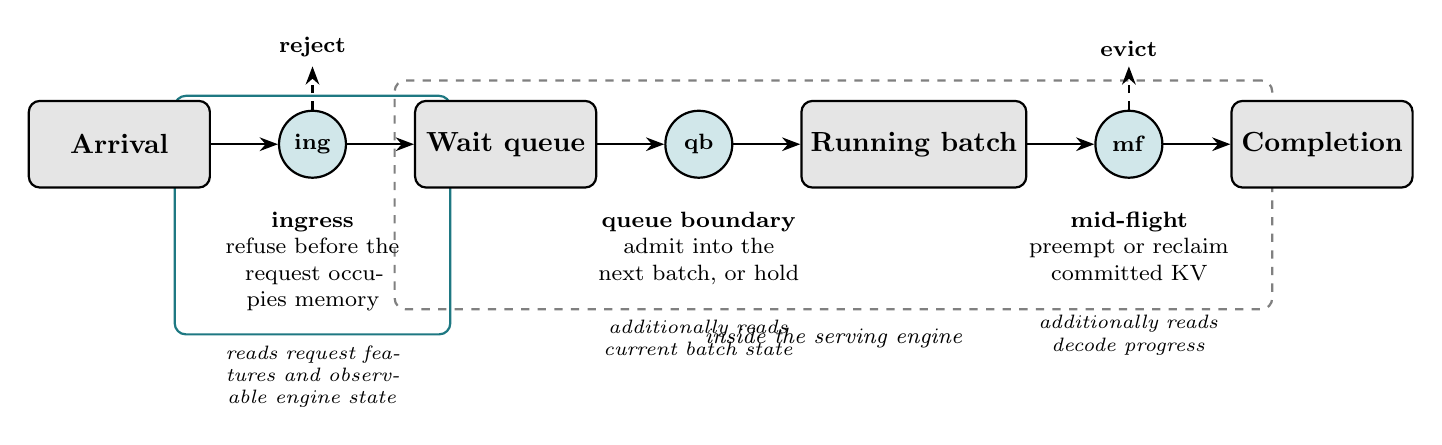
\begin{tikzpicture}[
  node distance=1.0cm and 1.1cm,
  stage/.style={rectangle, rounded corners, minimum width=2.3cm, minimum height=1.1cm, text centered, draw=black, thick, font=\bfseries, fill=admitgreylight},
  moment/.style={circle, draw=black, thick, minimum size=0.85cm, font=\bfseries\footnotesize, fill=admitteallight},
  arr/.style={-Stealth, thick, black},
  note/.style={font=\footnotesize, black, text width=2.9cm, align=center},
  sees/.style={font=\scriptsize\itshape, black, text width=3.0cm, align=center}
]

\node[stage] (arrive) {Arrival};
\node[moment, right=0.85cm of arrive] (ing) {\textsc{ing}};
\node[stage, right=0.85cm of ing] (wait) {Wait queue};
\node[moment, right=0.85cm of wait] (qb) {\textsc{qb}};
\node[stage, right=0.85cm of qb] (batch) {Running batch};
\node[moment, right=0.85cm of batch] (mf) {\textsc{mf}};
\node[stage, right=0.85cm of mf] (done) {Completion};

\draw[arr] (arrive) -- (ing);
\draw[arr] (ing) -- (wait);
\draw[arr] (wait) -- (qb);
\draw[arr] (qb) -- (batch);
\draw[arr] (batch) -- (mf);
\draw[arr] (mf) -- (done);

\node[note, below=0.3cm of ing] (ingn) {\textbf{ingress}\\refuse before the request occupies memory};
\node[note, below=0.3cm of qb] (qbn) {\textbf{queue boundary}\\admit into the next batch, or hold};
\node[note, below=0.3cm of mf] (mfn) {\textbf{mid-flight}\\preempt or reclaim committed KV};

\node[sees, below=0.2cm of ingn] {reads request features and observable engine state};
\node[sees, below=0.2cm of qbn] {additionally reads current batch state};
\node[sees, below=0.2cm of mfn] {additionally reads decode progress};

\node[above=0.55cm of ing, font=\footnotesize\bfseries] (rej) {reject};
\draw[arr, dashed] (ing.north) -- (rej.south);

\node[above=0.55cm of mf, font=\footnotesize\bfseries] (evict) {evict};
\draw[arr, dashed] (mf.north) -- (evict.south);

\begin{scope}[on background layer]
\node[fit=(ing)(ingn), draw=admitteal, thick, rounded corners, inner sep=5pt] {};
\node[fit=(wait)(qb)(batch)(mf)(mfn), draw=admitgrey, thick, dashed, rounded corners, inner sep=7pt] (inside) {};
\end{scope}
\node[font=\footnotesize\itshape, below=0.1cm of inside.south] {inside the serving engine};

\end{tikzpicture}%
}
\caption{Where an admission decision is taken. \textsc{ing} (ingress) acts before the request consumes engine memory, and reads only the request and whatever state the engine already exposes. \textsc{qb} (queue boundary) acts as the request is drawn into a batch and additionally reads batch state; \textsc{mf} (mid-flight) acts during decode and additionally reads the request's own progress. The later moments read more state, and in the systems surveyed here they are implemented inside the engine rather than in front of it.}
\label{fig:moments}
\end{figure}

Figure~\ref{fig:taxonomy} shows the two most-cited descriptive axes
(unit $\times$ SLO awareness) plotted against each other with
representative policies placed on the grid.

\begin{figure}[htbp]
\centering
\resizebox{0.9\textwidth}{!}{%
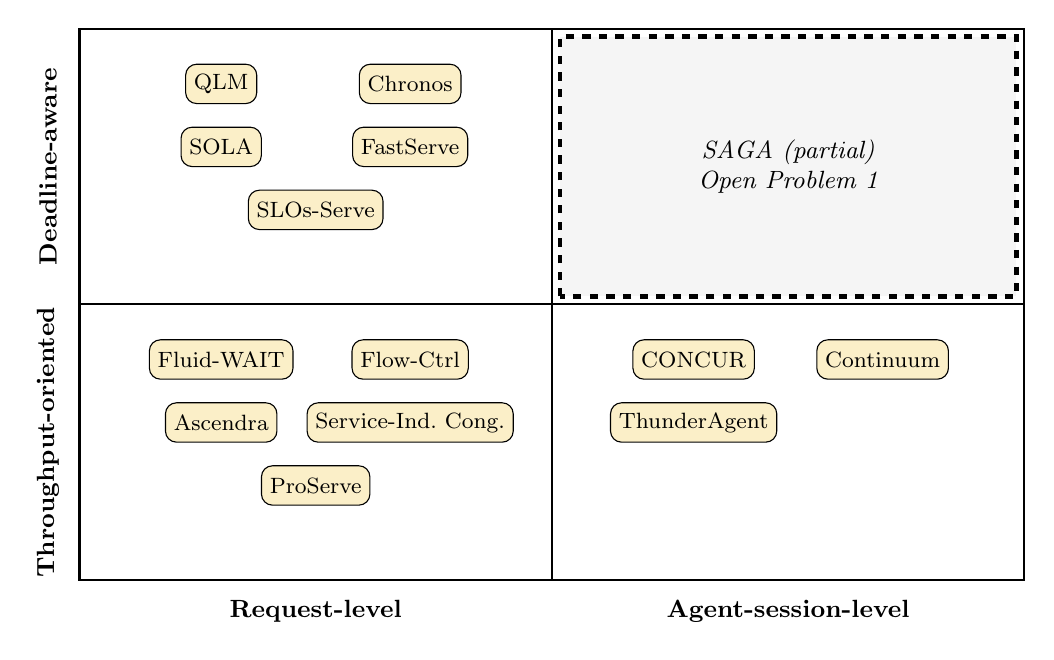
\begin{tikzpicture}[
  policy/.style={rectangle, rounded corners, minimum height=0.5cm, inner sep=3pt, fill=admityellowlight, draw=black, thin, font=\footnotesize},
  axislbl/.style={font=\bfseries\small},
  emptylbl/.style={font=\itshape\small, align=center}
]

% Frame
\draw[thick] (0, 0) rectangle (12, 7);
\draw[thick] (6, 0) -- (6, 7);
\draw[thick] (0, 3.5) -- (12, 3.5);

% Axis labels
\node[axislbl] at (3, -0.4) {Request-level};
\node[axislbl] at (9, -0.4) {Agent-session-level};
\node[axislbl, rotate=90] at (-0.4, 1.75) {Throughput-oriented};
\node[axislbl, rotate=90] at (-0.4, 5.25) {Deadline-aware};

% Q1: request x throughput
\node[policy] at (1.8, 2.8) {Fluid-WAIT};
\node[policy] at (4.2, 2.8) {Flow-Ctrl};
\node[policy] at (1.8, 2.0) {Ascendra};
\node[policy] at (4.2, 2.0) {Service-Ind.\ Cong.};
\node[policy] at (3.0, 1.2) {ProServe};

% Q2: agent x throughput
\node[policy] at (7.8, 2.8) {CONCUR};
\node[policy] at (10.2, 2.8) {Continuum};
\node[policy] at (7.8, 2.0) {ThunderAgent};

% Q3: request x deadline
\node[policy] at (1.8, 6.3) {QLM};
\node[policy] at (4.2, 6.3) {Chronos};
\node[policy] at (1.8, 5.5) {SOLA};
\node[policy] at (4.2, 5.5) {FastServe};
\node[policy] at (3.0, 4.7) {SLOs-Serve};

% Q4: empty
\draw[dashed, ultra thick, fill=admitgreylight!40] (6.1, 3.6) rectangle (11.9, 6.9);
\node[emptylbl] at (9, 5.25) {SAGA (partial)\\ Open Problem 1};

\end{tikzpicture}%
}
\caption{Policy taxonomy on Unit of admission (horizontal) $\times$
SLO awareness (vertical). The upper-right quadrant (agent-session
$\times$ deadline-aware) is partially occupied by SAGA
(arXiv:2605.00528), which satisfies agent-level scheduling and
per-task fairness but does not establish explicit TTFT/TBT
deadlines, online serving mode, or per-tenant fairness. This is the
seed for Open Problem~1.}
\label{fig:taxonomy}
\end{figure}



\subsection{Axis 1: Unit of admission}

Admission decisions can be made at three granularities.
\textbf{Request-level} (\textsc{unit-req}) policies admit or reject
each incoming prompt independently (QLM \citep{patke2024qlm}; Chronos
\citep{marref2026chronos}; FastServe \citep{wu2026fastserve}; SOLA
\citep{hong2025sola}). \textbf{Agent-session-level} (\textsc{unit-agt})
policies admit or reject entire multi-turn agent trajectories (CONCUR
\citep{chen2026concur}; Continuum \citep{li2026continuum}; ThunderAgent
\citep{kang2026thunderagent}). \textbf{Tenant-level} (\textsc{unit-ten})
policies gate admission per user or per organization (VTC
\citep{sheng2024vtc}).

\subsection{Axis 2: Setting}

Online serving handles interactive latency-sensitive workloads (most
of the field). Offline batch handles throughput-oriented inference
where per-request deadlines are relaxed. CONCUR is explicitly offline
per its ICML 2026 meta-review. Hybrid settings mix both.

\paragraph{Sub-branch: Concurrency context.}
We add a sub-branch after finding that Clairvoyant
\citep{sundaresan2026clairvoyant} solves an admission problem that
server-side policies cannot generalize to. Concurrent-batch servers
(vLLM, SGLang, TensorRT-LLM) admit at iteration granularity, contend
for KV blocks across many active requests, and can preempt mid-decode.
Serial edge backends (Ollama, llama.cpp) execute one request at a
time. Head-of-line blocking is the dominant tail-latency pathology at
the edge, and predictive shortest-job-first admission is the natural
response.

\subsection{Axis 3: SLO awareness}

Deadline-aware policies condition admission on TTFT or TBT bounds
(Chronos, SOLA, FastServe). Throughput-oriented policies maximize
aggregate goodput without per-request deadlines (CONCUR, Continuum).
Fairness-oriented policies enforce per-tenant or per-task equity (VTC,
FairBatching, Equinox). Cost-oriented policies minimize dollars or
energy per token.

\paragraph{Sub-branch: SLO granularity.}
SLOs-Serve \citep{chen2025slosserve} exposes a design axis nobody else
covers. Job-level SLOs specify a single deadline per multi-turn agent
job. Request-level SLOs specify one deadline per prompt (most of the
field). Per-stage SLOs specify distinct deadlines per stage of a
multi-turn application. Only SLOs-Serve models the per-stage case.

\paragraph{Sub-branch: Fairness type.}
Task-fairness allocates GPU cycles equitably between prefill and
decode tasks within one batch (FairBatching
\citep{lyu2025fairbatching}). Tenant-fairness equalizes served tokens
or SLO attainment across users (VTC \citep{sheng2024vtc}, Equinox
\citep{wei2025equinox}). These share no mechanism.

\subsection{Axis 4: Signal quantity}
\label{sec:axis-signal}

Every admission policy compares some measured quantity against a
threshold. Which quantity is the axis a practitioner can answer about
their own deployment without having read any of the policies, because it
asks what moves when their system is overloaded rather than how a given
paper is built. Across the sixteen admission-primary works the
quantities are:

\begin{description}[leftmargin=2em, itemsep=1pt]
\item[KV pressure] occupancy of the key-value cache, as a fraction of
      what the deployment has allocated (Fluid-WAIT, CONCUR, Continuum,
      AQUA).
\item[Queue depth] the number of requests waiting to enter a batch
      (QLM, FastServe, Fluid-WAIT, Continuum).
\item[Deadline slack] time remaining against a per-request target,
      compared with an estimate of time required (Chronos, SOLA,
      SLOs-Serve, Scorpio, ProServe).
\item[Predicted length] an estimate of how many tokens the request will
      generate, from a model over the prompt (FastServe, Scorpio,
      Clairvoyant).
\item[Wait estimate] a prediction of how long the request will queue,
      distinct from how many are queued (QLM).
\item[Batch state] the composition of the batch now forming, rather
      than a property of the arriving request (SOLA, FairBatching).
\item[Arrival rate] the offered load itself, with no engine-side
      quantity read (Flow-controlled scheduling).
\item[Analytic] no runtime signal: admission follows from a stability
      or reward argument (Service-Induced Congestion, Shen et al.).
\end{description}

The distribution matters for what the axis can do. Deadline slack and
KV pressure dominate, but they are not interchangeable: a deadline-slack
policy needs requests to arrive carrying deadlines, and a KV-pressure
policy needs the cache to actually fill. Section~\ref{sec:signal-predicts}
develops the second condition.

\paragraph{Sub-branch: Signal structure.} Orthogonal to which quantity
is read is how the policy combines readings into a decision. We identify
four structural forms, each with a short code we use throughout the
master classification (Table~\ref{tab:master}). The structure describes
policy design rather than deployment fit, so it is a sub-branch rather
than a primary axis: a reader cannot place their own system on it.

\textit{Scalar heuristics} (\textsc{sig-sca}) compare a single quantity
to a threshold (KV utilization for Fluid-WAIT; queue depth for QLM;
predicted output length for Clairvoyant).

\textit{Dual-gate conjunctions} (\textsc{sig-dg}) require multiple
signals to agree.
CONCUR declares congestion only when both KV utilization is high and
prefix cache hit rate is low, because high utilization with high hit
rate is healthy reuse rather than thrashing:
%
\begin{equation}
\text{congested} \;\iff\; \bigl(U_t > U_{\text{high}}\bigr) \,\wedge\, \bigl(H_t < H_{\text{thresh}}\bigr)
\label{eq:concur-dualgate}
\end{equation}
%
with fixed hyperparameters $U_{\text{high}} = 0.5$,
$H_{\text{thresh}} = 0.2$. Admission at agent granularity is adjusted
via additive-increase-multiplicative-decrease (AIMD) with $\alpha = 2$,
$\beta = 0.5$ per control interval.

\textit{Linear-program-based composite signals} (\textsc{sig-lp}) treat
admission as one variable in a joint optimization. QLM formulates a linear program over
virtual queues, minimizing total SLO-violation penalty:
%
\begin{equation}
\min \; \sum_{i \in \mathcal{R}} \max\bigl(0,\; W_{q,i} - \mathrm{SLO}_i\bigr)
\label{eq:qlm-lp}
\end{equation}
%
subject to one-to-one request-group-to-position and model-transition
constraints; solvable in about 5\,s at 400{,}000 queued requests using
Gurobi.

\textit{Formal worst-case-response-time bounds} (\textsc{sig-wcrt})
derive an admission test from real-time-systems theory. Chronos casts prefill as a
sporadic job with worst-case execution time proportional to input
length, then derives the closed-form bound
%
\begin{equation}
R_i \;\le\; \frac{\rho_P \cdot D_{\text{TTFT}}}{1 - \rho_P} + p_i(\alpha B + \gamma), \qquad \rho_P < 1
\label{eq:chronos-wcrt}
\end{equation}
%
where $\rho_P$ is prefill utilization, $D_{\text{TTFT}}$ is the TTFT
deadline, $p_i = \lceil \ell_i / B \rceil$ is the number of chunks,
$\alpha$ is prefill kernel throughput, $B$ is chunk size, and $\gamma$
is fixed overhead. Algorithm~1 of \citep{marref2026chronos} rejects on
arrival if $\rho_P \ge 1$, if the bound exceeds the TTFT deadline, or
if a TBT capacity check fails.

\subsection{Axis 5: Portability}
\label{sec:axis-portability}

The four axes above describe what a policy decides. This one describes
what it costs to run, and it is the axis a practitioner is likely to
apply first, because it can eliminate candidates before any question of
fit arises.

\textbf{Class A} policies decide from the arriving request and state the
engine already exposes: cache occupancy, queue length, counts of running
and waiting requests. Such a policy can sit in front of an unmodified
engine, as a proxy or gateway, and is deployable by anyone who can route
traffic.

\textbf{Class B} policies need to influence which requests enter a
batch, or to act on requests already decoding. That cannot be done from
outside: it requires changes inside the engine's scheduler, and in
practice a maintained fork.

The split follows from the decision moment
(\S\ref{sec:taxonomy}, folded): \textsc{ing} is Class A, while
\textsc{qb} and \textsc{mf} are Class B. Of the sixteen
admission-primary works, ten are Class A and six are Class B. A reader
who cannot maintain an engine fork is choosing among ten, not sixteen,
and that is knowable before reading any of them.

No paper in the corpus states its own class. It is derivable from the
mechanism each describes, which is why we treat it as an axis rather
than as reported metadata: the information is present in the text but
never surfaced as a deployment property.

\subsection{What the Signal axis predicts}
\label{sec:signal-predicts}

The Signal axis has a consequence for how published results should be
read. A policy discriminates by comparing a measured quantity against a
threshold, so it can discriminate only when that quantity varies over
the operating range of the deployment. Where the signal is effectively
constant, the comparison returns the same answer for every arrival, and
the policy admits or refuses uniformly regardless of how its threshold
is set. Its observable behaviour in that case matches an uncontrolled
baseline.

The two cases are not distinguishable from a results table. A policy
whose signal never approached its threshold and a policy that evaluated
a varying signal and declined to reject will report the same admission
counts and the same downstream latencies. Separating them requires the
observed range of the signal over the evaluation. We did not find that
range reported in any paper we examined (Section~\ref{sec:items},
item~3).

This also bounds what the present survey can establish. Which
deployments hold which signals constant depends on the engine, the
model, and the workload, and is an empirical question rather than a
bibliographic one. We do not answer it here, and we are not aware of
published measurements that do; it is stated as Open Problem~7.

\subsection{Placing the corpus, and where it fails}
\label{sec:placement}

We applied the taxonomy to all sixteen admission-primary works,
recording seven properties for each: the five axes, plus what the
policy assumes an arriving request carries, plus the range its signal
took during the paper's own evaluation. The last two are not axes. They
are recorded because a reader needs both to act on the taxonomy: a
deadline-slack policy is unusable on traffic that carries no deadlines,
and a reported result is uninterpretable if the signal behind it never
moved. The exercise is a test of the axes as much as of the corpus,
since an axis that cannot be filled from the published text is not one
a reader could use.

Six of the seven fill, and all five axes are among them. Every paper states its unit and setting; every
paper's objective is recoverable; the quantity each policy reads is
always identifiable, even where the paper does not name it as a signal;
and the portability class follows from the mechanism in all sixteen
cases. Eight of the sixteen require nothing of an arriving request
beyond the request itself, five require a deadline or SLO class, two
require a session identifier, and one requires a priority class.

One property does not fill. For no paper in the corpus could we
determine the range the policy's own signal took during its evaluation.
A threshold that was never approached and a threshold that was
approached but not crossed produce the same admission counts and the
same downstream latencies, so no reported number distinguishes a policy
that was exercised from one that was merely present.

The consequence for a reader is narrow and specific. The taxonomy will
tell you which policies could apply to your deployment. It will not tell
you whether the published evidence for any of them describes a policy
that was actually exercised, because that evidence is not reported.
Section~\ref{sec:items} states the property as the third of seven
reporting items, and Section~\ref{sec:open} states the measurement it
would take to establish which of those items are load-bearing.

\subsection{The unclaimed intersection}

Plotting the corpus (Figure~\ref{fig:taxonomy}) shows that
agent-level $\times$ online $\times$ deadline-aware $\times$
per-tenant-fair is not fully occupied by any published policy.
CONCUR is agent-level but offline and throughput-oriented. Chronos
is deadline-aware but request-level. FairBatching is fair but
task-level not tenant-level. SAGA
\citep{guo2026saga} is the closest work: it schedules at the
agent-workflow level with a bounded-deviation Agent Fair Share
metric and reports 99.2\% SLO attainment, but the paper does not
establish that Agent Fair Share reduces to per-tenant fairness in
multi-user settings, does not decompose the SLO into TTFT and TBT,
and does not commit to an online-serving mode. We treat SAGA as a
partial occupant and preserve OP1 as an open problem for the
subset (agent + online + TTFT+TBT + per-tenant) that no published
work satisfies simultaneously.

Re-deriving this after adding the portability axis leaves the cell
empty, and surfaces a second gap beneath it. Among the sixteen
admission-primary works, two are agent-level: CONCUR, which is Class A
but offline and throughput-oriented, and Continuum, which is online but
Class B and optimises job completion time rather than a deadline. So
within the admission-primary set there is no agent-level policy that
both serves online traffic and deploys without an engine fork. A reader
running multi-turn agent workloads who cannot maintain a fork has no
candidate at all, which is a sharper statement than the empty
intersection and follows from a property no paper reports about itself.

We state this for the admission-primary set only. ThunderAgent
\citep{kang2026thunderagent} is agent-level and coded at ingress, which
would occupy the cell, but its mechanism is program-level residency with
eviction from high-bandwidth memory, and whether that is deployable
outside the engine is not something we have established. It is the
near-miss a reader should check first.

\section{Method}
\label{sec:method}

We conducted a systematic review following an adapted PRISMA 2020
workflow. Figure~\ref{fig:prisma} shows the identification,
screening, eligibility, and inclusion counts.

\begin{figure}[htbp]
\centering
\resizebox{0.85\textwidth}{!}{%
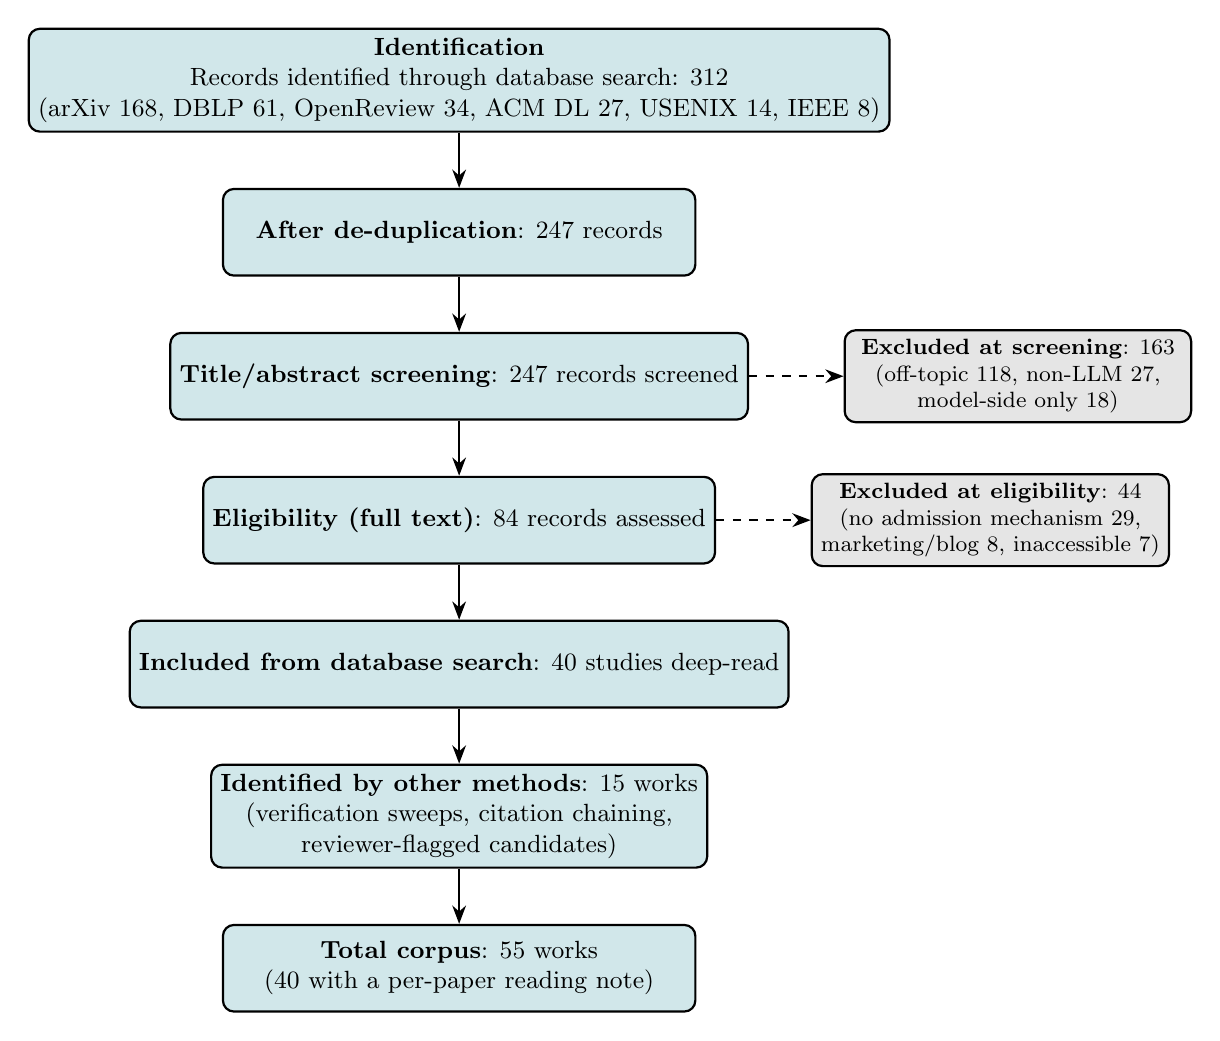
\begin{tikzpicture}[
  node distance=0.7cm,
  stage/.style={rectangle, rounded corners, minimum width=6cm, minimum height=1.1cm, text centered, draw=black, thick, font=\small, fill=admitteallight, align=center},
  excl/.style={rectangle, rounded corners, minimum width=4.4cm, minimum height=1.1cm, text centered, draw=black, thick, font=\footnotesize, fill=admitgreylight, align=center},
  arr/.style={-Stealth, thick, black},
  side/.style={-Stealth, thick, black, dashed}
]

\node[stage] (ident) {\textbf{Identification}\\Records identified through database search: 312\\(arXiv 168, DBLP 61, OpenReview 34, ACM DL 27, USENIX 14, IEEE 8)};
\node[stage, below=of ident] (dedup) {\textbf{After de-duplication}: 247 records};
\node[stage, below=of dedup] (screen) {\textbf{Title/abstract screening}: 247 records screened};
\node[stage, below=of screen] (elig) {\textbf{Eligibility (full text)}: 84 records assessed};
\node[stage, below=of elig] (incl) {\textbf{Included from database search}: 40 studies deep-read};
\node[stage, below=of incl] (other) {\textbf{Identified by other methods}: 15 works\\(verification sweeps, citation chaining,\\reviewer-flagged candidates)};
\node[stage, below=of other] (total) {\textbf{Total corpus}: 55 works\\(40 with a per-paper reading note)};

\node[excl, right=1.2cm of screen] (exs) {\textbf{Excluded at screening}: 163\\(off-topic 118, non-LLM 27,\\model-side only 18)};
\node[excl, right=1.2cm of elig] (exe) {\textbf{Excluded at eligibility}: 44\\(no admission mechanism 29,\\marketing/blog 8, inaccessible 7)};

\draw[arr] (ident) -- (dedup);
\draw[arr] (dedup) -- (screen);
\draw[arr] (screen) -- (elig);
\draw[arr] (elig) -- (incl);
\draw[arr] (incl) -- (other);
\draw[arr] (other) -- (total);
\draw[side] (screen.east) -- (exs.west);
\draw[side] (elig.east) -- (exe.west);

\end{tikzpicture}%
}
\caption{PRISMA 2020 flow for the admission-control corpus. Counts as
of 2026-09-11. Search protocol and per-paper protocol described in the
subsections below.}
\label{fig:prisma}
\end{figure}


\paragraph{Search dates and sources.} Search dates ran from May 2022
(Orca) through September 2026. Sources: DBLP; arXiv (cs.DC, cs.LG,
cs.OS, cs.PF categories); OpenReview forums for ICLR, NeurIPS, ICML,
MLSys; USENIX conference proceedings for OSDI, NSDI, ATC, FAST; ACM
Digital Library for SOSP, SoCC, ASPLOS, EuroSys, SIGMETRICS; IEEE
Xplore for HPCA, ISCA; Google Scholar for cross-reference discovery.

\paragraph{Search strings.} Admission-control terms (``admission
control'', ``queue management'', ``load shedding'', ``request
rejection'', ``request dropping'', ``SLO-aware admission'',
``throttling'', ``backpressure'', ``gating'') were combined with
LLM-serving terms (``LLM inference'', ``LLM serving'', ``language
model inference'', ``agentic inference'', ``continuous batching'',
``KV cache''). Boolean expansion followed each hit's related-work
section for backward-citation discovery.

\paragraph{Inclusion.} A paper was included if all four conditions
held: (i)~published or preprinted between 2022-05-01 and 2026-09-11;
(ii)~primary application domain is LLM inference (not general DNN
serving or generic queueing theory); (iii)~either admission control is
the primary contribution, or the paper is a top-venue scheduling /
KV-management / fairness work whose mechanism has direct
admission-adjacency; (iv)~full text was accessible via arXiv HTML,
venue PDF, or OpenReview.

\paragraph{Exclusion.} A paper was excluded if any held: (i)~pure
model-side optimization (quantization, pruning, distillation) without
a serving-time admission component; (ii)~vision or speech inference
without LLM applicability; (iii)~marketing materials or blog posts
without a peer-reviewed or arXiv-preprint anchor.

\paragraph{Tier structure.} We organized the corpus into six tiers
based on admission-primacy. Tier~1 (16 papers): admission-primary,
one policy per paper. Tier~2 (11 papers): queueing theory or
fairness-primary with admission-adjacency. Tier~3 (6 papers):
KV-cache-management papers whose mechanism has admission
implications. Tier~4 (10 papers): top-venue scheduling papers with
admission as a secondary or missing component. Tier~5 (7 papers):
foundational works cited for background. Tier~6 (5 papers): prior
broad surveys used for differentiation. The six tiers sum to the
fifty-five works of the corpus, of which forty carry a per-paper
reading note.

\paragraph{Per-paper protocol.} For each work we recorded venue,
authors, arXiv or DOI identifier, code availability, taxonomy
placement across all five axes, primary contribution, baseline set,
evaluation setup (model, engine, workload, hardware), claimed headline
numbers with configuration qualifiers, fidelity notes, and open
questions surfaced. Notes were written in a common markdown template
to make cross-work comparison tractable. The complete per-paper corpus
is public at the survey's artifact repository.

\paragraph{Reviewer discussion evidence.} For several open problems
(Section~\ref{sec:open}) we cite public OpenReview discussion or venue
meta-reviews as evidence that a gap is practitioner-recognized. Where
a peer reviewer explicitly asked a question that the paper's rebuttal
did not answer, we treat that as grounded evidence for an open
problem.

\paragraph{Non-experiments.} We did not run experiments. Where papers
report conflicting numbers, we report each source's number as stated
with the operating-point qualifier the source specifies, and flag the
conflict rather than adjudicate.

\section{Policy clusters}
\label{sec:clusters}

\subsection{Request-level SLO-aware admission}

QLM \citep{patke2024qlm} is the canonical peer-reviewed
admission-primary paper for online serving. It maintains virtual
queues per model and formulates request scheduling as the linear
program in Equation~\ref{eq:qlm-lp}. A Request Waiting Time Estimator
predicts per-request wait using Central Limit Theorem bounds over
historical output-token distributions. Reported improvements are 40 to
90 percent SLO attainment lift and 20 percent (single-model) to 400
percent (multi-model) throughput gain over vLLM and EDF baselines on a
heterogeneous 30 A10 plus 50 A100 cluster serving Mistral-7B,
Vicuna-13B, and LLaMA-70B on ShareGPT. Code is public at
\url{https://github.com/QLM-project/QLM}.

Chronos \citep{marref2026chronos} derives a formal schedulability
condition (Equation~\ref{eq:chronos-wcrt}) for LLM inference. On a 7B
model in a discrete-event simulator against 50{,}000 sampled Azure
conversational-service requests, the reported separation is
load-dependent. At 5$\times$ nominal load Chronos and the uncontrolled
schedulers all reach 0.00 percent TTFT miss, and the difference is in
tail latency and admission volume: Chronos admits 88.9 percent at a P99
TTFT of 161 ms, against 100 percent admitted at 400 ms for FCFS and
EDF. At 10$\times$ load the uncontrolled schedulers collapse to 99.44
percent TTFT miss while Chronos holds 0.00 percent by admitting 53.9
percent. Rate limiting alone does not reproduce this: a
throughput-matched token bucket (AC-FCFS) misses 15.40 percent at that
same 53.9 percent admission, and 6.80 percent at the 5$\times$
operating point despite matching Chronos's admission volume there. The
comparison is therefore a case for the formal test over rate matching
rather than over scheduling as such. Simulator code
is public at \url{https://github.com/am-research/rtss-ttft-tbt}.

SOLA \citep{hong2025sola} formalizes fine-grained scheduling as an LP
over per-request and systemic state. Empirical scheduling raises SLO
attainment from 45.5 percent to 99.4 percent and serves 1.04-1.27
$\times$ more requests. The constraint-relaxation mechanism at the
$\alpha$-percentile is an implicit admission decision hidden inside a
scheduler.

FastServe \citep{wu2026fastserve} argues for token-granularity
preemption rather than reject-on-arrival admission. The 31.4$\times$
average-latency throughput improvement is measured on OPT-175B across
16 A100 GPUs against vLLM v0.1.7 on ShareGPT. Code is public but runs
on the SwiftTransformer engine.

SLOs-Serve \citep{chen2025slosserve} is the only paper in our corpus
that handles per-stage-of-agent SLOs. Multi-SLO DP admits requests
whose joint SLOs are attainable and declines the rest through soft
admission. Reports 2.2$\times$ geometric-mean per-GPU serving capacity
across six workload scenarios and five models.

ProServe \citep{huang2025proserve} frames scheduling as unified
multi-priority request scheduling. Admission emerges from the
SlideBatching loop's budget-and-memory gates combined with a
token-level deadline-aware gain function
$f_{\text{TDG}}(r) = \sum_i w_r(i) \cdot
\mathbb{I}[t_{r,i} < \tau_{\text{TTFT}} + (i-1)\tau_{\text{TPOT}}]$
that scores requests against their per-token deadlines. This is
queue-boundary admission (\textsc{qb}) rather than pure ingress, and
we classify it as such in Table~\ref{tab:master}. Baselines include
vLLM-FCFS, Sarathi-FCFS, Sarathi-Priority, Weighted VTC, and
FairBatching. No code released.

Scorpio \citep{tang2026scorpio} is the most recent admission-primary entry
and splits the decision across three stages: admission, queue
management, and batch selection. Its TTFT Guard reorders by least
deadline first and rejects requests whose first-token deadline is
unattainable, estimating attainability from the cumulative prefill time
of everything already queued. Its TPOT Guard admits only when the
predicted per-token latency for the resulting virtual batch stays under
the tightest TPOT target in the running set. Both guards read a
predicted output length from a fine-tuned OPT-125M classifier over 100
bins, which places Scorpio in the dual-gate signal class with learned
rather than analytic grounding. It is evaluated on vLLM with
Llama-3.1-8B and Gemma-2-27B on four A100s, against vLLM, S3 and
Mooncake, reporting up to 14.4 times goodput and 46.5 percent better SLO
adherence under high load.

Two details matter beyond those numbers. First, Mooncake is itself an
early-rejection admission mechanism, which makes Scorpio one of the few
policy-versus-policy comparisons in the corpus
(Table~\ref{tab:baselines}). Second, Scorpio computes goodput with every
arriving request in the denominator, so a rejected request counts as an
SLO miss. That is the discipline we adopt in
Section~\ref{sec:defs} for goodput-under-admission, arrived at
independently. A metric counting only admitted requests flatters
shedding: refuse 95 percent of traffic, serve the rest perfectly, and it
reads 100 percent. Two efforts converging on the same denominator by
separate routes is the strongest argument available that it is the
correct one.

\subsection{Agent-session-level admission}

CONCUR \citep{chen2026concur} identifies middle-phase thrashing in
agentic batch inference. The controller applies the dual-gate
condition of Equation~\ref{eq:concur-dualgate}. Headline gains are
4.09$\times$ throughput against SGLang on Qwen3-32B at 256 sessions,
tensor parallelism 8, on 8 H100 GPUs, and 1.90$\times$ against SGLang
on DeepSeek-V3 at 40 sessions, TP 16, 16 H100 GPUs. Against Continuum
as a baseline, CONCUR shows 1.69$\times$ on Qwen3-32B (added in
rebuttal). The meta-review states the paper targets offline
throughput-oriented inference and that online serving is out of scope.

Continuum \citep{li2026continuum} manages KV retention rather than
gating admission. Per-session time-to-live is set by maximizing
expected benefit minus cost. Reports 1.12-3.66$\times$ JCT improvement
across Llama-3.1, Gemma-3, and GLM-4.5 on SWE-Bench, BFCL, and
OpenHands, with an internal-deployment peak of 8.18$\times$. Public
vLLM fork at \url{https://github.com/Hanchenli/vllm-continuum}.

ThunderAgent \citep{kang2026thunderagent} treats disk, ports, and
sandboxes as first-class scheduled resources alongside GPU. A central
scheduler pauses and restores programs with explicit state migration.
Integrated into NVIDIA Dynamo 2.0.

SAGA \citep{guo2026saga} schedules at the level of the entire agent
workflow rather than per inference call, introducing Agent Execution
Graphs that capture workflow structure across tool-call boundaries
and predict KV cache reuse. The paper defines Agent Fair Share, a
task-completion-time fairness metric with provable bounded-deviation
guarantees, and reports 99.2\% SLO attainment under multi-tenant
interference. Admission is described as ``session-affinity batching
with work stealing'' at the scheduler level; whether this reduces to
ingress admission is not established, and per-tenant fairness (as
opposed to per-task fairness) is not evaluated. We classify SAGA as
agent-level, mid-flight, scalar-signal in Table~\ref{tab:master}.
See Section~\ref{sec:open} OP1 for the sharpened residual open
problem.

\subsection{Fairness-aware admission and scheduling}

VTC \citep{sheng2024vtc} formalizes LLM-serving fairness through a
cost function over tokens processed rather than requests, with default
weights $w_p = 1$ for input and $w_q = 2$ for output. The theoretical
guarantee bounds service difference between any two
continuously-backlogged clients:
%
\begin{equation}
|W_f - W_g| \;\le\; 2 \max\bigl(w_p \cdot L_{\text{input}},\; w_q \cdot M\bigr)
\label{eq:vtc-bound}
\end{equation}
%
where $M$ is the max batch size, with a matching lower bound of
$w_q \cdot M$ proving the 2$\times$ constant is tight. Empirically VTC
halves max unfairness versus FCFS while matching throughput (779
versus 777 tok/s on 27 Chatbot Arena clients), whereas RPM(5) rate
limiting collapses throughput to 340 tok/s. Artifact-evaluated code at
\url{https://github.com/Ying1123/VTC-artifact}.

FairBatching \citep{lyu2025fairbatching} attacks fairness between
prefill and decode tasks within a batch. Achieves 2.29$\times$ tail
latency reduction, 20 percent single-node capacity improvement, and
54.3 percent cluster-level capacity improvement. Implementation is
only 90 lines of invasive vLLM changes.

Equinox \citep{wei2025equinox} argues that equal tokens do not imply
equal user experience. Requires a Model of Prediction Ensemble to
predict output length, latency, throughput, and GPU utilization per
prompt. Thirteen percent fairness improvement measured against
Equinox's own metric.

FairServe \citep{khan2024fairserve}, from Microsoft on real Copilot
production traces, combines Online Interaction Throttling (OIT) at
ingress with Weighted Service Counting (WSC) for scheduling. OIT
throttles at the LLM-interaction level when the KV cache is
overloaded, and WSC selects requests from users who have received
the least service, weighted by application priority. Reports
1.03--1.06$\times$ TTFT latency reduction. FairServe is the only
work in our corpus that operates at the user/application-interaction
level rather than at request, agent-session, or organizational
tenant granularity; we classify it as tenant-level with a dagger
(\S\ref{sec:master}) and note that it does not decompose SLOs into
TTFT+TBT deadlines. Source code not released as of paper
submission.

\subsection{Queueing-theoretic and algorithmic}

Service-Induced Congestion \citep{ao2026sic} provides the theoretical
justification (Section~\ref{sec:whyhard},
Equation~\ref{eq:throughput-bound}).

Flow-Controlled Scheduling \citep{dong2026flowcontrolled} proves
necessary and sufficient stability conditions using a static
token-bucket. LIFO eviction inverts fairness for interactive
workloads.

Fluid-WAIT \citep{ao2025fluidwait} derives a threshold admission rule
from a fluid-model equilibrium.

Shen et al.\ \citep{shen2026twolayer} prove $\tilde{O}(\sqrt{K T})$
regret for joint online configuration selection and admission control
under an i.i.d.\ reward-resource assumption per configuration:
%
\begin{equation}
\text{Reg}^{\text{mix}}(T) \;\le\; C_1 \alpha \sqrt{K T \cdot d \log T} + C_2 \sqrt{T \log T} + K R_{\max}
\label{eq:shen-regret}
\end{equation}
%
The paper motivates via LLM serving but validates empirically on
Alibaba cluster traces.

Jaillet et al.\ \citep{jaillet2026online} target online scheduling
under KV-cache constraints with monotonically growing per-request
memory. Their memory-cognizant policies achieve competitive-ratio
bounds under structured arrivals plus $\alpha$-accurate predictions.

Mitzenmacher and Shahout \citep{mitzenmacher2025queueing} enumerate 25
open problems at the intersection of queueing theory and LLM serving.

Clairvoyant \citep{sundaresan2026clairvoyant} is the sole entry in the
serial-edge concurrency-context sub-branch. Predictive
shortest-job-first using an XGBoost classifier over 19 lexical
features delivers 70 to 76 percent short-request $p_{50}$ latency
reduction on an RTX 4090.

Ascendra \citep{ikram2025ascendra} uses an SLO-risk predictor to
promote requests between low-priority and high-priority queues.

Niyama \citep{goel2025niyama} sits adjacent to admission rather than
inside it. It co-schedules mixed workloads on shared infrastructure with
fine-grained QoS classes and a hybrid fairness-efficiency priority
policy, and under overload it applies selective request relegation,
degrading service for lower classes rather than refusing work at the
door. We include it because relegation and admission answer the same
question with different verbs, and because its overload behaviour is
directly comparable to that of a deferring admission policy.

\subsection{KV-cache management adjacent}

KVFlow \citep{pan2025kvflow} is pure cache management with
steps-to-execution ranking over SGLang's radix tree. No admission
logic. Complementary to CONCUR, not a substitute.

Cake \citep{jin2025cake} optimizes single-request TTFT via hybrid
compute-versus-load KV decisions.

InferCept \citep{abhyankar2024infercept} chooses between preserving,
swapping, and discarding KV during tool-call intercepts. Cost model
prices GPU-memory-bytes-times-time locally; does not account for
queue length, which Continuum identifies as its key limitation.

Pie \citep{gim2025pie} provides a programmable serving substrate with
generation-loop handlers and KV page management. No cross-inferlet
scheduler API and no admit-reject hook.

\subsection{Scheduling papers with admission-adjacent components}

We audited the nine LLM serving systems that the admission-primary
papers in this corpus most often build on or compare against, published
between 2022 and 2026. The selection rule is that dependency rather
than a venue list: these are the engines and schedulers the rest of the
literature treats as its substrate. They happen to appear at OSDI,
SOSP, NSDI, ASPLOS, EuroSys, MLSys and HPCA, which is a consequence of
where such work is published rather than a criterion we applied.

Table~\ref{tab:9for9} summarizes what each does under overload. All
nine locate the overload response inside the engine, redistributing
work through batching, migration, placement, autoscaling or memory
management. None takes a decision at the ingress, and none sets out to:
these are scheduling and memory-management contributions, and refusing
work at the door lies outside the design space each paper defines for
itself. The observation is about where research attention has gone, not
about a shortcoming in these systems.

The distinction that matters here is engine-level against
infrastructure-level, and it does not track venue. Token Pools
\citep{cunningham2026tokenpools} gates at the API boundary and is a
control-plane contribution rather than an engine one; it is in this
corpus and classified in Table~\ref{tab:master}. Reading the two
together, ingress admission appears where a system owns the boundary in
front of the fleet, and not in the engine papers, whichever venue
either is published at. We would draw the same conclusion had Token
Pools appeared at any of the seven.

\begin{table}[htbp]
\centering
\caption{Overload response mechanisms in the nine LLM serving systems the admission literature most often builds on, 2022--2026. Each locates its overload response inside the engine; the ingress-admission column is empty across all nine, which reflects the scope each paper sets rather than an omission. Token Pools, a control-plane contribution rather than an engine one, does gate at the API boundary and is discussed separately.}
\label{tab:9for9}
\small
\rowcolors{2}{white}{admitgreylight!40}
\begin{tabular}{l l l l}
\toprule
\rowcolor{admitteallight}
\textbf{Paper} & \textbf{Venue} & \textbf{Overload mechanism} & \textbf{Ingress admission?} \\
\midrule
Orca & OSDI 2022 & FCFS + KV-slot cap (implicit) & No \\
Sarathi-Serve & OSDI 2024 & Chunked prefill batching & No \\
Llumnix & OSDI 2024 & Live request migration & No \\
DistServe & OSDI 2024 & P/D disaggregation, static split & No \\
Past-Future \citep{pastfuture2025} & ASPLOS 2025 & Memory projection at batch boundary & Internal only \\
Aegaeon \citep{aegaeon2025} & SOSP 2025 & Per-token autoscaling & No \\
Jenga \citep{jenga2025} & SOSP 2025 & Memory heterogeneity mgmt & No \\
AdaServe \citep{adaserve2026} & EuroSys 2026 & SLO-customized spec decode & No \\
PASCAL \citep{pascal2026} & HPCA 2026 & Runtime phase detection & No \\
\bottomrule
\end{tabular}
\end{table}

Past-Future's memory-projection gate is the closest of the nine to
admission, and it operates on already-queued requests rather than at
ingress. Taken with Token Pools, which gates at the API boundary, the pattern suggests that ingress
admission has been treated as an infrastructure concern rather than an
engine-level research question. That is the gap this survey addresses:
not that these systems are missing something they should have, but that
the decision they leave to the deployment has received little
systematic study.

\paragraph{Token Pools (CAIS 2026): partial counter-example.}
Cunningham \citep{cunningham2026tokenpools} introduces token pools, a
control-plane abstraction expressing capacity as inference-native
entitlements (token throughput, KV cache, concurrency). Admission is
enforced at the API boundary: ``The auth service intercepts every
request before it reaches the backend. On each request, it validates
the API key against an entitlement... and makes an admission decision
based on multiple factors.'' Requests whose priority falls below the
admission threshold ``are rejected with HTTP 429 and a
\texttt{Retry-After} header, allowing clients to back off gracefully.'' The same entitlements drive autoscaling
decisions through a unified capacity model, directly addressing our
Open Problem~5 (coupling admission and autoscaling). The evaluation
is single-node (DGX Spark, Qwen3-8B) with no released code, so we
rate the evidence \textsc{m}. Token Pools tightens but does not close
the engine-level gap: it sits outside the nine
OSDI/SOSP/NSDI/ASPLOS/EuroSys/MLSys/HPCA set, and its evaluation
scale is orders of magnitude below what those venues typically
require.

\section{Master classification}
\label{sec:master}

Table~\ref{tab:master} classifies twenty-eight of the fifty-five works
in the corpus along the three orthogonal
taxonomy levels (Unit, Moment, Signal grounding), plus a
GRADE-adapted evidence rating for the strength of empirical support
behind each work's headline claims. Unit codes: \textsc{req} request,
\textsc{agt} agent-session, \textsc{ten} tenant. Moment codes:
\textsc{ing} ingress, \textsc{qb} queue boundary, \textsc{mf}
mid-flight (during decode). Signal codes: \textsc{sca} scalar,
\textsc{dg} dual-gate, \textsc{lp} linear-program, \textsc{wcrt}
formal worst-case-response-time bound.

\paragraph{What the table does not classify.} Twenty-seven corpus works
carry no row. Twelve are foundational systems, textbooks, or prior
surveys, for which an admission taxonomy is not defined. Nine are
engine-level scheduling papers that contain no admission
mechanism to classify, which is the nine-of-nine finding of
Section~\ref{sec:clusters} rather than an omission here. The remaining
six are AQUA \citep{kumar2025aqua}, Chiron, Mooncake, Niyama
\citep{goel2025niyama}, Throughput-Optimal Scheduling and Beyond
Prediction, each of which touches admission indirectly:
AQUA and Mooncake through reclamation and early rejection, Chiron
through autoscaling, Niyama through relegating lower QoS classes rather
than refusing them, and the last two through queueing-theoretic results
that do not specify a decision rule. Mooncake warrants a specific
note, since it states a ``prediction-based early rejection policy'' and
appears as a baseline in Table~\ref{tab:baselines}. We leave it
unclassified on the narrower ground that admission is a component of a
disaggregation architecture rather than the paper's contribution: the
rejection policy is described but not evaluated as a policy, with no
ablation isolating its effect and no comparison against an alternative
admission rule. It is therefore an admission mechanism we can name but
not place on the Signal axis with the same evidence we have for the
entries in Table~\ref{tab:master}.

\paragraph{GRADE rubric (operationalized).}
We assign each work one of four evidence levels using four criteria:
(1)~evaluation medium (real hardware vs simulator vs theoretical);
(2)~number of independent baselines evaluated;
(3)~code availability (public + artifact-evaluated vs public
unevaluated vs closed); (4)~workload realism (production trace or
public benchmark vs synthetic). A work is assigned:
\begin{description}[leftmargin=1.5em, itemsep=1pt]
\item[\textsc{h} (high)] real hardware, three or more independent
      baselines including at least one from a different venue,
      artifact-evaluated public code, and evaluation on a public
      benchmark or production trace.
\item[\textsc{m} (moderate)] real hardware, at least one independent
      baseline, public code (not necessarily artifact-evaluated), and
      either a public benchmark or a well-documented synthetic
      workload.
\item[\textsc{l} (low)] simulator-only, or unreleased code, or
      single-baseline against an unnamed reference, or synthetic
      workload without documented parameters.
\item[\textsc{vl} (very low)] position paper, tutorial, or
      theoretical result without empirical evaluation.
\end{description}
The rubric is stricter than reviewer-perceived at borderline cells.
QLM earns \textsc{h} because its artifact is Artifact-Evaluated,
baselines include vLLM+EDF and SHEPHERD, and evaluation runs on
Chatbot-Arena traces on a heterogeneous 80-GPU cluster. Chronos
earns \textsc{m} rather than \textsc{h} because the evaluation is
simulator-only despite artifact release. VTC earns \textsc{h}
because the OSDI artifact evaluation and clean cross-baseline
comparison satisfy all four criteria. Per-paper justifications are
included in the artifact repository's per-paper coding sheet.

\begin{table}[htbp]
\centering
\caption{Master classification of admission-primary and admission-adjacent works. See legend above the table for codes. ``$-$'' means the axis does not apply.}
\label{tab:master}
\small
\setlength{\tabcolsep}{4pt}
\rowcolors{2}{white}{admitgreylight!40}
\resizebox{\textwidth}{!}{%
\begin{tabular}{l l l c c c c}
\toprule
\rowcolor{admitteallight}
\textbf{System / Paper} & \textbf{Venue} & \textbf{Year} & \textbf{Unit} & \textbf{Moment} & \textbf{Signal} & \textbf{GRADE} \\
\midrule
\multicolumn{7}{l}{\textit{Request-level SLO-aware admission (\S\ref{sec:clusters})}} \\
QLM                     & SoCC       & 2024 & req & ing & lp   & H \\
Chronos                 & Frontiers CS & 2026 & req & ing & wcrt & M \\
SOLA                    & MLSys      & 2025 & req & mf  & lp   & M \\
FastServe               & NSDI       & 2026 & req & mf  & sca  & M \\
SLOs-Serve              & preprint   & 2025 & req & ing & lp   & L \\
Fluid-WAIT              & preprint   & 2025 & req & ing & sca  & L \\
Scorpio                 & WISE       & 2026 & req & ing & dg   & M \\
Ascendra                & preprint   & 2025 & req & qb  & sca  & L \\
Flow-Ctrl scheduling    & preprint   & 2026 & req & ing & wcrt & L \\
Service-Induced Cong.   & preprint   & 2026 & req & ing & wcrt & M \\
Jaillet et al.\         & preprint   & 2026 & req & ing & lp   & M \\
Shen et al.\            & ICML       & 2026 & req & ing & lp   & M \\
ProServe \citep{huang2025proserve} & preprint & 2025 & req & qb & lp & L \\
\midrule
\multicolumn{7}{l}{\textit{Agent-session-level admission}} \\
CONCUR                  & ICML       & 2026 & agt & ing & dg   & M \\
Continuum               & ICLR WS    & 2026 & agt & mf  & sca  & M \\
ThunderAgent            & ICML       & 2026 & agt & ing & sca  & L \\
SAGA                    & preprint   & 2026 & agt & mf  & sca  & L \\
\midrule
\multicolumn{7}{l}{\textit{Fairness-oriented}} \\
VTC                     & OSDI       & 2024 & ten & mf  & sca  & H \\
FairBatching            & preprint   & 2025 & req & mf  & sca  & L \\
Equinox                 & preprint   & 2025 & ten & ing & sca  & L \\
FairServe               & preprint   & 2024 & ten$^\dagger$ & ing & dg  & M \\
\midrule
\multicolumn{7}{l}{\textit{Gateway-level admission + autoscaling}} \\
Token Pools             & CAIS       & 2026 & ten & ing & lp   & M \\
\midrule
\multicolumn{7}{l}{\textit{Serial-edge concurrency context}} \\
Clairvoyant             & preprint   & 2026 & req & ing & sca  & L \\
\midrule
\multicolumn{7}{l}{\textit{KV-management adjacent (no ingress admission)}} \\
KVFlow                  & NeurIPS    & 2025 & $-$ & mf  & sca  & M \\
Cake                    & ICML       & 2025 & $-$ & mf  & sca  & M \\
InferCept               & ICML       & 2024 & $-$ & mf  & sca  & M \\
Pie                     & SOSP       & 2025 & $-$ & mf  & $-$  & L \\
\midrule
\multicolumn{7}{l}{\textit{Position / tutorial}} \\
Mitzenmacher \& Shahout & SIGMETRICS & 2025 & $-$ & $-$ & $-$  & VL \\
\bottomrule
\end{tabular}%
}
\end{table}

The nine scheduling papers from the OSDI/SOSP/NSDI/ASPLOS/EuroSys/
nine engine-level systems (Orca, Sarathi-Serve, Llumnix,
DistServe, Past-Future, Aegaeon, Jenga, AdaServe, PASCAL) are
omitted from Table~\ref{tab:master} because none includes an
ingress-level admission decision at all; they are summarized
separately in Table~\ref{tab:9for9}. TokenScale
\citep{lai2025tokenscale} is also omitted despite its LLM-serving
scope: careful reading confirms it is a pure autoscaling framework
(Token Velocity signal drives prefiller/decoder scaling only) with
no admission-control component. Chiron \citep{patke2025chiron} is a
hierarchical autoscaler with no admission component and appears
only under Open Problem~5.

\paragraph{Dagger note on FairServe.} FairServe
\citep{khan2024fairserve} operates at the user- and
application-interaction level rather than at any of our three
canonical unit codes (\textsc{req}, \textsc{agt}, \textsc{ten}). We
mark it \textsc{ten}$^\dagger$ because a Microsoft-CoPilot
``application'' is closer to a tenant than to an individual request
or agent session, but the classification is genuinely lossy for
this work; readers checking the four-property intersection should
note that FairServe satisfies the online axis and a weighted
per-user fairness axis, but does not decompose SLOs into TTFT and
TBT deadlines and does not operate at the agent-session level.
Placement was chosen after considering the reviewer's explicit
question 3 on the four-property intersection.

\section{Admission-signal overhead synthesis}
\label{sec:overhead}

The corpus supports one cross-paper empirical synthesis that no
individual paper reports: the tradeoff between the \emph{cost} of
computing an admission signal at ingress and the \emph{goodput lift}
that signal delivers over a first-come-first-serve baseline. We call
this the \emph{admission-signal overhead}. Five anchor points from
the corpus are shown in Table~\ref{tab:overhead}, each carrying its
operating point verbatim from the source paper so that the reader
can see the heterogeneity of contexts across which we are reasoning.

\begin{table}[htbp]
\centering
\caption{Admission-signal overhead: cost of computing an admission decision (per request, best-case) versus lift reported in the source paper over that paper's own FCFS baseline. Every row reports the exact operating context from its source; \textbf{no normalization is applied across rows} and cross-row comparison is not justified without head-to-head evaluation.}
\label{tab:overhead}
\small
\setlength{\tabcolsep}{4pt}
\rowcolors{2}{white}{admitgreylight!40}
\resizebox{\textwidth}{!}{%
\begin{tabular}{l l l l l l}
\toprule
\rowcolor{admitteallight}
\textbf{Anchor (signal class)} & \textbf{Model / engine} & \textbf{Hardware} & \textbf{SLO tuple / workload} & \textbf{Cost} & \textbf{Lift over FCFS} \\
\midrule
Fluid-WAIT (\textsc{sig-sca}) & Llama-2-7B / vLLM & 1$\times$A100 40 & TTFT 500\,ms / synthetic Poisson & tens of \textmu s & 10--20\% goodput \\
Clairvoyant (\textsc{sig-sca}) & Llama-3.1-8B / Ollama & RTX 4090 & p50 latency / ShareGPT & tens of \textmu s & 70--76\% short-request p50 latency reduction \\
CONCUR (\textsc{sig-dg}) & Qwen3-32B / SGLang & 8$\times$H100 & JCT / BrowserComp, 256 sessions & $<$100\,\textmu s + AIMD update & 4.09$\times$ throughput vs SGLang \\
QLM (\textsc{sig-lp}) & Mistral-7B + Vicuna-13B + LLaMA-70B / vLLM & 30$\times$A10 + 50$\times$A100 & TTFT tail / ShareGPT & $\approx$5\,s Gurobi solve at 400\,K queued & 40--90\% SLO-attainment vs vLLM; 20\% throughput single-model, 50--400\% multi-model, vs vLLM+EDF \\
Chronos (\textsc{sig-wcrt}) & 7B ref.\ model / discrete-event sim & simulator & TTFT deadline / 50\,K Azure requests & \textmu s (closed-form) & TTFT miss 99.44\%$\rightarrow$0.00\% at 5$\times$ load (sim) \\
\bottomrule
\end{tabular}%
}
\end{table}

\paragraph{What Table~\ref{tab:overhead} does and does not support.}
The five anchors span different models, engines, hardware, SLO
definitions, and workloads. Reading down the ``Lift'' column suggests
that costlier signals return larger lifts, but this pattern is
\emph{directional at best} because every anchor is a
different-workload single-baseline comparison to that anchor's own
FCFS. We explicitly do not claim: (a) a functional form of cost
versus lift; (b) a crossover point beyond which additional signal
complexity ceases to pay off; (c) that any pair of anchors would
retain its ordering under head-to-head evaluation. The synthesis is
provided so the reader can see the shape of the tradeoff and the
absence of normalized evidence for it.

\paragraph{GRADE certainty.} We rate this synthesis \textsc{low}
using the rubric in Section~\ref{sec:master}. Each anchor cites its
source paper's own numbers under that paper's own operating point;
no head-to-head comparison exists in the literature
(Table~\ref{tab:baselines}). Closing this identification gap is what
the reporting items in Section~\ref{sec:repro} are meant to enable, and
establishing which of them are load-bearing is Open Problem~7
(Section~\ref{sec:open}).

\section{Reproducibility and comparison methodology}
\label{sec:repro}

We audited public code availability across our corpus, scoped to the
tiers where releasing an implementation is a well-formed expectation.
Seven of the sixteen admission-primary papers have released code as of
September 2026 (QLM, Chronos, FastServe, Shen et al., Continuum,
Clairvoyant, AQUA), as have five of the six KV-cache-adjacent works
(KVFlow, InferCept, Pie, ThunderAgent, Cake) and one of the ten
fairness and queueing-theory works (VTC). Two qualifications apply to
the admission-primary count: Chronos released a discrete-event
simulator rather than a real-engine implementation, and AQUA is
included in this corpus as the canonical preemption-based foil to
admission control rather than as an admission policy itself.

These rates are higher than the ``reproducibility crisis'' framing
common in prior surveys would suggest, and the adjacent literature
releases code more often than the admission literature does. We report
rates per tier rather than a single corpus-wide figure because the full
corpus includes foundational works, textbooks and prior surveys, for
which code release is not a meaningful expectation; a denominator
spanning them would not be interpretable.

The more consequential gap is at the methodology level.
Table~\ref{tab:baselines} shows the baseline set used by each
admission-primary paper. No two papers share a baseline \emph{set}. Six baselines recur across
more than one paper, and the recurrence is concentrated in comparators
that are not admission policies: vLLM in six papers and Sarathi in
four, then EDF and FCFS twice each. Only two of the six are admission
mechanisms, and one of those, AC-FCFS, is a token bucket constructed
as an ablation rather than a published system. That leaves SHEPHERD as
the single published admission policy any two papers have in
common.

\begin{table}[htbp]
\centering
\caption{Baseline overlap across admission-primary papers. The most-used baseline (vLLM) appears in six papers and Sarathi in four; no other appears in more than two; and no two papers share the same baseline set. Read by what the columns contain: vLLM, SGLang, Sarathi, DistServe and Orca are serving engines, so a tick there measures a policy against the absence of admission control rather than against an alternative to it, and EDF, FCFS and SJF are classical disciplines rather than published systems. SOLA's Sarathi entry is marked \emph{re-impl.} because it reimplements chunked prefill on vLLM rather than comparing against upstream Sarathi-Serve. Among published admission systems, SHEPHERD \citep{shepherd2023} is used as a baseline by two papers (QLM and Ascendra); AC-FCFS also appears twice, but it is a throughput-matched token bucket constructed as an ablation rather than a system published in its own right. Scorpio's comparison against Mooncake is the corpus's clearest instance of one admission mechanism measured against another. Rows for CONCUR, Continuum, SAGA, and Token Pools are also omitted from column headers (a paper cannot baseline against itself); Continuum appears only as CONCUR's rebuttal-added comparator. Empty rows for SAGA and Token Pools indicate baselines that are not extractable from the current text of those preprints.}
\label{tab:baselines}
\small
\setlength{\tabcolsep}{4pt}
\rowcolors{2}{white}{admitgreylight!40}
\resizebox{\textwidth}{!}{%
\begin{tabular}{l *{12}{c}}
\toprule
\rowcolor{admitteallight}
\textbf{Paper} & \textbf{vLLM} & \textbf{SGLang} & \textbf{Sarathi} & \textbf{DistServe} & \textbf{Orca} & \textbf{EDF} & \textbf{FCFS} & \textbf{SJF} & \textbf{SHEPHERD} & \textbf{Weighted VTC} & \textbf{Continuum} & \textbf{AC-FCFS} \\
\midrule
QLM (SoCC 2024)          & \checkmark &            &            &            & (cite)     & \checkmark & (impl.) &            & \checkmark &            &            &            \\
CONCUR (ICML 2026)       &            & \checkmark &            &            &            &            &         &            &            &            & \checkmark & \checkmark \\
Chronos (Frontiers 2026) &            &            &            &            &            & \checkmark & \checkmark &         &            &            &            & \checkmark \\
SOLA (MLSys 2025)        & \checkmark &            & re-impl.   &            &            &            &         & \checkmark &            &            &            &            \\
FastServe (NSDI 2026)    & \checkmark &            &            &            &            &            &         &            &            &            &            &            \\
SLOs-Serve (2025)        & \checkmark &            & \checkmark & \checkmark &            &            &         &            &            &            &            &            \\
FairBatching (2025)      &            &            & \checkmark &            &            &            &         &            &            &            &            &            \\
Ascendra (2025)          &            &            &            &            &            &            &         &            & \checkmark &            &            &            \\
ProServe (2025)          & \checkmark &            & \checkmark &            &            &            & \checkmark &         &            & \checkmark &            &            \\
SAGA (2026)              & \multicolumn{12}{l}{(baselines not extractable from preprint abstract; body-text extraction failed via WebFetch)} \\
Token Pools (CAIS 2026)  & \multicolumn{12}{l}{(single-node evaluation; no external policy baselines reported)} \\
Fluid-WAIT (2025)        & \multicolumn{12}{l}{(unnamed ``widely used baselines'')} \\
Scorpio (WISE 2026)      & \checkmark & \multicolumn{11}{l}{\ + S3 and Mooncake, the latter itself an early-rejection mechanism} \\
\bottomrule
\end{tabular}%
}
\end{table}

Reading the literature top to bottom, a practitioner cannot answer
``which admission policy wins on my workload.''

\subsection{Seven reporting items that vary across the corpus}
\label{sec:items}

Reading the corpus for what would be needed to place a result against a
deployment, seven properties recur as the points of divergence. Six are
reported inconsistently. The seventh, the observed range of the signal
the policy reads, we did not find reported by any of the sixteen
admission-primary papers.

That asymmetry is worth stating plainly, because it is not what we
expected to find. Placing all sixteen papers on the axes of
Section~\ref{sec:taxonomy} succeeds on every axis but one: unit,
setting, SLO-awareness, the quantity the policy watches, the metadata a
request must carry, and whether the policy is deployable in front of an
unmodified engine are all recoverable from the published text. Ten of
the sixteen are deployable without modifying the engine; eight require
nothing of a request beyond the request itself. Selection fails on a
single missing fact, and it is the fact that determines whether a
reported improvement is interpretable at all.

All seven concern disclosure of what was done rather than prescription
of what to run, so none of them asks a paper to change its evaluation.

\begin{enumerate}[leftmargin=1.5em, itemsep=2pt]
\item \textbf{Capacity-relative load}. Offered load expressed as a
      multiple of the deployment's measured serveable capacity, rather
      than as a raw arrival rate or an unquantified ``high load''. Two
      papers reporting the same arrival rate on different hardware may
      be operating in different regimes.
\item \textbf{Calibrated deadlines}. SLO targets expressed relative to
      unloaded latency on the same model and hardware. The difficulty
      of meeting a fixed millisecond target varies with the deployment,
      so absolute targets are not comparable across papers.
\item \textbf{Signal liveness}. The observed range of the quantity the
      policy reads, over the evaluation. Not one of the sixteen
      admission-primary papers reports it.\footnote{This is an absence
      across the evaluation sections we extracted, not a guarantee that
      no paper mentions a range anywhere. We recorded each paper's
      evaluation setup, including the quantity its policy reads; none
      stated the range that quantity took. A figure axis showing, say,
      cache occupancy over time would arguably satisfy the item and
      would not have been captured by this procedure.} Without it, a policy whose signal never approached its
      threshold cannot be distinguished from one that evaluated a
      varying signal and declined to reject
      (Section~\ref{sec:signal-predicts}).
\item \textbf{Repeats and spread}. The number of repeats and the
      observed spread, rather than a single run or a median alone.
\item \textbf{Parameter provenance}. For each parameter, whether it was
      fitted on the evaluated deployment, inherited from the source
      paper, or left at a default. Policies carrying hardware-dependent
      cost constants cannot otherwise be reproduced.
\item \textbf{Metric definition}, in particular the goodput
      denominator: whether rejected requests count as misses
      (Definition~\ref{def:goodput}) or are excluded. The two
      conventions yield different numbers for the same run, and the
      difference grows with the rejection rate.
\item \textbf{Configuration disclosure}. Model, engine version,
      hardware, workload subset, offered load, SLO tuple, and the
      identity of the baseline actually run.
\end{enumerate}

We do not claim this set is minimal or sufficient, or that its items
matter equally; it records where the corpus diverges, stated so that a
reader can check a paper against it. Determining which of the seven are
load-bearing, in the sense that omitting one allows a reported result to
move without a reader detecting the change, is not answerable by
reading. It requires running the same policy under controlled variation
of each item in turn, and we state it as Open Problem~7.

Per-paper coding sheets, taxonomy placements, and inclusion and
exclusion decisions for this survey are released with it, to support
third-party audit and to reproduce the master table
(\artifacturl).

\section{Production evidence}
\label{sec:prod}

Real inference-fleet incidents map directly onto admission failure
modes. Table~\ref{tab:incidents} lists seven public postmortems and
identifies the leading signal that would have prevented each. Each
row carries a source URL and a confidence annotation:
\textsc{v}~(verified) means the failure mode is explicitly named in
the linked postmortem; \textsc{i}~(inferred) means the failure mode
is our reading of an official postmortem whose wording is looser.

\begin{table}[htbp]
\centering
\caption{Production incidents mapped to admission signals. Confidence: V verified from postmortem; I inferred from postmortem. Every row cites a postmortem that is public at the time of writing.}
\label{tab:incidents}
\scriptsize
\setlength{\tabcolsep}{3pt}
\rowcolors{2}{white}{admitgreylight!40}
\resizebox{\textwidth}{!}{%
\begin{tabular}{p{2.6cm} p{3.6cm} p{2.6cm} p{3.2cm} p{2.8cm} c}
\toprule
\rowcolor{admitteallight}
\textbf{Incident} & \textbf{Failure mode} & \textbf{Trusted signal (was)} & \textbf{Leading signal (needed)} & \textbf{Source} & \textbf{Conf.} \\
\midrule
OpenAI DALL$\cdot$E queue collapse & Work admitted past client cancellation timeout & Queue depth & Queue age at admission & \citep{openai_dalle_postmortem} & I \\
OpenAI Nov 8 2023 & Routing nodes crossed soak point; adding replicas insufficient & Utilization & Rate of change of utilization & \citep{openai_nov2023} & V \\
OpenAI Dec 11 2024 & Telemetry API storm; stale DNS for 20\,min then failed at TTL expiry & Aggregate utilization dashboards & Control-plane health independent of data-plane cache & \citep{openai_dec2024} & V \\
OpenAI Apr 2025 & Control-plane OOM; failover overloaded second cluster; misleading errors & Cluster availability & Correct 429/503 propagation on failover & \citep{openai_apr2025} & V \\
Anthropic Jan 21 2026 & Insufficient compute for demand; latency then errors for $\sim$90\,min & Metrics dashboard refresh cycle & Sub-minute capacity-constraint detection & \citep{anthropic_jan2026} & I \\
Anthropic Aug 29 2025 & LB moved short-context traffic to servers configured for 1M-token contexts & Pool-level utilization & Per-configuration utilization decomposition & \citep{anthropic_aug2025} & V \\
Anthropic HTTP 529 semantics & Provider-overloaded distinct from client-rate-limited & Single 429/503 signal & Dedicated 529 semantics & \citep{anthropic_api_errors} & V \\
\bottomrule
\end{tabular}%
}
\end{table}

\subsection{Practitioner checklist}

For operators evaluating an admission policy: (i)~what does the policy
admit against, and can that signal be corrupted by the failure modes
in Table~\ref{tab:incidents}? (ii)~does the policy return 429, 503, or
529, and does the choice match your client retry logic? (iii)~how
quickly does the policy respond to a capacity change smaller than your
metric-dashboard refresh interval? (iv)~does the policy see
per-configuration utilization, or only pool-level averages?

\section{Open problems}
\label{sec:open}

Seven high-signal open problems. Each cites concrete evidence from
either published peer review or the primary source's own limitations.

\paragraph{Relation to the existing agenda.} Mitzenmacher and Shahout
\citep{mitzenmacher2025queueing} enumerate roughly twenty-five open
problems across queueing with predictions, dynamic batching, adaptive
scheduling, GPU orchestration, compound AI systems and reasoning
workloads. Ours are not disjoint from theirs and we do not claim they
are: OP4 and their reasoning-workload section address the same
workload, and OP6 sits inside the queueing-theoretic territory their
paper defines. The difference is in what is being asked. Their list is
a theoretical agenda, stating problems whose resolution would be a
result: how prediction error should be modelled, when Gittins policies
are implementable, what SOAP analysis extends to. Ours are questions
about evidence, stating gaps whose resolution would be a measurement or
a system: which admission policy suits which deployment, whether an
omitted reporting item lets a result move undetected. A reader wanting
the theory agenda should take theirs; this list is what the published
systems literature leaves unestablished.

\paragraph{OP1: Agent-level admission with per-tenant fairness under online arrivals.}
The CONCUR reviewer discussion at ICML 2026 (OpenReview
\texttt{mmdqUrEY24}) contains this exchange: Reviewer Afcg maintained
a weak-accept score with the final justification ``the underlying
problem can be addressed through more effective request-level
scheduling.'' CONCUR added a Continuum comparison in rebuttal but did
not add a request-level baseline. SAGA
\citep{guo2026saga} partially closes the gap by scheduling at agent
workflow granularity with a bounded-deviation Agent Fair Share
metric, but the paper does not evaluate per-tenant fairness across
concurrent users, does not decompose SLOs into TTFT and TBT, and
does not commit to an online serving mode. The sharpened open
problem is: an agent-level policy that admits under online arrivals,
respects both TTFT and TBT deadlines per stage, and provides
proven per-tenant (not per-task) fairness bounds.

\paragraph{OP2: Online serving admission for agentic workloads.}
The CONCUR meta-review states the paper targets offline
throughput-oriented agentic inference. Continuum and ThunderAgent
also target offline batch. SAGA reports online SLO attainment but
does not evaluate under bursty arrivals with reject/defer accounting.
An admission policy for agentic workloads that maintains stable
goodput under Poisson-plus-burst arrivals and reports
reject/defer/admit rates with per-agent-class breakdown remains
open.

\paragraph{OP3: Multi-tenant admission with per-tenant SLOs.}
VTC handles fairness in served tokens. FairBatching handles fairness
between prefill and decode. Neither handles per-tenant deadline SLOs
with tenant-aware admission.

\paragraph{OP4: Reasoning-trace-aware admission at ingress.}
PASCAL addresses phase-aware scheduling for reasoning-augmented LLMs,
but its phase detection is entirely runtime. Ingress-level
reasoning-versus-chat classification is unclaimed.

\paragraph{OP5: Cross-validation of coupled admission and autoscaling.}
Chiron autoscales replicas; QLM (same research group) does
per-replica SLO-aware queueing. Token Pools
\citep{cunningham2026tokenpools} directly couples entitlement-based
admission with autoscaling, but the evaluation is single-node
(DGX Spark, Qwen3-8B) with no released code, so the interaction
regime is unmeasured at cluster scale. The residual open problem
becomes: cross-validate a Token-Pools-style coupled admission +
autoscaling policy against QLM + Chiron on the same multi-model
multi-tenant cluster trace.

\paragraph{OP6: Formal schedulability with LLM-specific WCRT.}
Chronos derives closed-form WCRT bounds under a linear kernel model
with roofline-derived parameters, never measured on real silicon.
Probabilistic WCET analysis and mixed-criticality models are open.

\paragraph{OP7: Which reporting items are load-bearing?}
Seven of the sixteen admission-primary papers have released code, which
weakens the ``no artifacts'' framing. The remaining obstacle to
comparison is the absence of a shared account of what must be reported
for two results to be read against each other.
Section~\ref{sec:items} identifies seven items that diverge across the
corpus. Their identification does not establish that they matter.

The open problem is to determine, for each item, whether omitting it
permits a reported result to move without a reader detecting the
change. Answering it requires running a fixed policy on a fixed
deployment under controlled variation of each item in turn, and
observing whether the headline number moves while the paper's
disclosure stays constant. An item for which no such variation can be
constructed would not be load-bearing, and the set should shrink
accordingly.

Item~3 (signal liveness) is the clearest case to test, since we found
no paper reporting it at all. The question there is whether the omission
changes what a reader should conclude. Establishing
that requires running a policy whose signal is known to be inert
alongside one whose signal is known to move, on the same deployment and
against the same trace, and asking whether any reported number separates
them.

\section{Threats to validity}
\label{sec:threats}

\paragraph{The central finding is bibliographic, not empirical.} We
report that no paper in the corpus states the observed range of the
quantity its policy reads, and that this is what prevents a reader from
telling a policy that could not act from one that chose not to. The
first half is an absence in what we extracted; the second is an
argument. Neither is a measurement. We did not run the policies, and we
do not claim to have observed a policy failing this way in a
deployment. Establishing that would require running a policy whose
signal is known to be inert alongside one whose signal is known to
move, on the same deployment and against the same trace, and it is
stated as Open Problem~7 for that reason.

The absence itself has a specific shape. We recorded each paper's
evaluation setup, including the quantity its policy compares against a
threshold, and no paper stated the range that quantity took during the
evaluation. A paper reporting it somewhere we did not extract, a figure
axis showing cache occupancy over time for instance, would not have
been captured. The claim is therefore that we did not find it, over a
defined extraction procedure, rather than that it does not exist.

\paragraph{Screening and coding were done by one reader.} Systematic
review methodology ordinarily calls for at least two independent coders
and a reported agreement statistic. This review had one. Inclusion
decisions, tier assignments and axis placements therefore carry no
inter-rater reliability measure, and a second coder might place
borderline works differently. Three specific placements are known to be
contestable and are marked as such in the text: FairServe, whose
user-and-application granularity does not fit any of our three unit
codes; SAGA, which we treat as a partial occupant of the unclaimed
intersection; and Mooncake, which states an early-rejection policy but
does not evaluate it as one. To make disagreement checkable rather than
invisible, the per-paper coding sheets are released with the survey
(\artifacturl).

\paragraph{The corpus boundary involves judgment.} Admission-adjacent
is not a sharp category. Works that relegate rather than refuse, that
reclaim memory rather than decline requests, or that autoscale rather
than gate, all answer the overload question with a different verb. We
included Niyama on those grounds and excluded TokenScale on the
opposite ones, and Appendix~\ref{sec:excluded} lists every work
considered and set aside with the reason. A reviewer who disagrees with
a particular call can see which one it was.

\paragraph{The reporting items are identified, not validated.} Section
\ref{sec:items} names seven properties that recur as points of
divergence. We do not claim the set is minimal, that its members are
independent, or that they matter equally. Whether omitting any one of
them lets a reported result move undetected is a question about
measurement, and it is the open problem this survey hands on rather
than one it settles.

\paragraph{Coverage has a date and a venue boundary.} The search ran
through September 2026. Admission-primary work is appearing quickly,
and a survey of a moving subfield is a snapshot. The nine-paper slice
in Section~\ref{sec:clusters} is drawn from seven venues; work at other
venues, and industrial deployment reports in particular, is covered
where we found it but was not systematically swept.

\section{Conclusion}
\label{sec:conc}

Admission control for LLM inference serving is a distinct sub-problem
that governs whether downstream batching, KV management, and
preemption have the capacity headroom to succeed. Between 2022 and
2026 the field produced thirteen admission-primary works at
peer-reviewed top venues plus one accepted workshop paper and more
than a dozen preprints. We surveyed fifty-five works across
admission-primary, admission-adjacent, and scheduling clusters.

Our five-axis taxonomy with four sub-branches organizes the corpus
without redundancy. The intersection agent-level $\times$ online
$\times$ (TTFT+TBT-deadline-decomposed) $\times$ per-tenant-fair
remains unoccupied; SAGA is a partial occupant on the agent-level
and fairness axes only (Figure~\ref{fig:taxonomy}).

The nine engine-level systems the admission literature builds on
place their overload response
inside the engine rather than at the ingress
(Table~\ref{tab:9for9}); Token Pools (CAIS 2026) sits outside this
slice and does gate at the gateway.
Production postmortems
(Table~\ref{tab:incidents}) show that overload originating from a
mis-specified admission signal propagates faster than downstream
batching, migration, or autoscaling can absorb, so these techniques
are insufficient on their own.

Reproducibility of individual artifacts is higher than commonly
framed, at seven of the sixteen admission-primary papers.
Reproducibility of cross-paper comparison is essentially zero
(Table~\ref{tab:baselines}). The seven reporting items in
Section~\ref{sec:items} are what would enable closing it.

Seven open problems each carry either public peer-review evidence or
the primary source's own limitation statement. The most tractable
candidates for near-term progress are OP1 (agent-level admission
with per-tenant fairness under online arrivals, sharpened by SAGA
as partial occupant), OP2 (online admission for agentic workloads
with reject/defer accounting), OP5 (cross-validation of coupled
admission and autoscaling on top of Token Pools), and OP7 (which
reporting items are load-bearing).

\appendix
\section{Works considered and set aside}
\label{sec:excluded}

Two categories, kept separate because the evidence behind them differs.

\paragraph{Examined and excluded.} Read in full, then excluded with a
stated reason.

\begin{itemize}[leftmargin=1.5em, itemsep=2pt]
\item \textbf{TokenScale} \citep{lai2025tokenscale}. A pure autoscaling
      framework: its Token Velocity signal drives prefiller and decoder
      scaling only. The full text contains no instance of admission,
      admit, reject, refuse or shed; the single mention of dropping
      requests is in related work, describing other systems and
      explicitly contrasting them with TokenScale.
\item \textbf{Mooncake} \citep{qin2025mooncake} is included in the
      corpus but deliberately not placed in
      Table~\ref{tab:master}. It states a ``prediction-based early
      rejection policy'', so it is an admission mechanism we can name,
      but the policy is described rather than evaluated: there is no
      ablation isolating its effect and no comparison against an
      alternative admission rule. Placing it on the Signal axis would
      assert an evidential basis the paper does not provide.
\end{itemize}

\paragraph{Identified but not examined.} Surfaced during verification
searches in September 2026 and not read in full, so not classified. We
list them because a reader working in this area will encounter them,
and because an unexamined candidate is a more useful thing to disclose
than to omit.

\begin{itemize}[leftmargin=1.5em, itemsep=2pt]
\item \textbf{OmniServe} \citep{omniserve2026} reached our candidate
      list through a search snippet describing it as regulating
      admissions. Checking the abstract does not support that reading:
      it describes CPU-GPU attention piggybacking for co-located
      latency-sensitive and best-effort loads, together with ``a
      dynamic batching control policy to adapt to fluctuating request
      arrivals''. Batching control governs how queued requests are
      grouped, which is a different decision from whether a request is
      admitted. We record it here because the snippet was persuasive
      and the correction is the kind a reader may otherwise repeat,
      and because we have not read the full paper and cannot rule out
      an admission mechanism in its body.
\item Agent-side candidates: Adaptive Memory Admission Control for LLM
      Agents, Agent Control Protocol, and ConsistencyGate, each
      described in its abstract as performing admission at agent
      granularity. These bear on the unclaimed intersection of
      Section~\ref{sec:taxonomy}, which is an agent-level claim, and
      any of them could occupy or narrow it.
\item Multi-tenant and attribution work: Token Latency Fairness,
      LLMVisor, and AgentServeSim.
\end{itemize}

The second list is a statement about this survey's coverage rather than
about those works. It is given so that the boundary of what was read is
visible, and so that the agent-level claims in particular are read with
the knowledge that three unexamined candidates bear on them.



\bibliographystyle{unsrtnat}
\bibliography{references}

\end{document}
